\chapter{Learning Power Compensations}
\label{cha:learning_power_compensations}

\minitoc

This Chapter proposes the introduction of Reinforcement Learning (RL) to choose the best compensation policy. We previously saw that the heuristics proposed (Next, Peak, Last, and Workload) have good results compared to just following the plan. The best heuristic depends on the workload and power production. So, the idea is to let RL algorithms learn which are the best policies to use at each different moment inside the three-day time window. The following sections will describe our approach to solving the compensation problem. First, we start presenting the algorithms used in this section to compare with the previous results. Then, we define the state, action, and rewards. Finally, we present the results and a discussion.

\section{Reinforcement Learning}

As mentioned in Chapter \ref{cha:related_work}, Reinforcement Learning (RL) performs a trial-and-error approach, where an agent explores an environment, takes actions, and receives feedback \cite{kaelbling1996reinforcement}. Three components compose an RL model: \textbf{state}, \textbf{actions}, and \textbf{reward}. Let's exemplify it, by using RL to define the content of a website. A website can apply RL to define which content to display for every user. The idea is to discover the user's subject preferences (e.g., sports, politics, technology, etc.) The \textbf{state} is the information about the user, such as age, previous subjects read, etc. Using this \textbf{state}, the RL evaluates it and chooses the articles to show to the user. The chosen articles' subjects are the \textbf{actions}. Finally, the \textbf{reward} can be 1 if the user clicked on the article and 0 if the user did not click on it. RL algorithm tries to maximize (in this case) the \textbf{reward}, increasing the number of clicks. Since RL does not know the user's behavior, it tries some articles. The clicked articles reinforce the user's subject preferences. Then, the following process is performed at each decision moment (see Figure \ref{fig:reinforcement}):
\begin{enumerate}
    \item RL receives a state from the environment;
    \item RL verifies which action to take for this state;
    \item RL applies the action in the environment;
    \item The environment returns a reward for this action;
    \item RL uses the reward to calculate the relation between state and action;
    \item The environment goes to a new state, restarting the process.
\end{enumerate}

The RL interacts with the environment in this way several times. RL uses the feedback (reward) to learn which are the best actions for the states. Another important aspect is the exploration-exploitation. Since in the early interactions, the RL agent does not know the environment, it starts exploring the different actions in the state. After some interactions, the agent stops the exploration and starts to exploit the actions with higher rewards in the past. Different approaches can be used to model the exploration-exploitation transition, which also depends on the RL algorithm. In this thesis, we used two reinforcement learning algorithms: Q-Learning and Contextual Multi-Armed Bandit. Section \ref{sec:RL_algos} present them. However, before presenting the algorithms, we describe the state, action, and rewards definition. Our objective with RL is to define: \textit{where to compensate the power difference (positive or negative) for each step within a three-day time window?} For example, the best actions in the early steps can be to put the power in the steps with a higher power deficit, but not too much to not dry the battery too fast. So, RL must find a balance between the actions. For ease the comprehension, this chapter uses the following terms:
\begin{itemize}
    \item \textit{Decision step}: The step that takes action to modify the power of a future step. It will receive a reward according to the impact of this action. It can impact only one future step;
    \item \textit{Future step}: The step that receives more or less power from one or several decision steps. When this future step finishes, it is possible to give back a reward for the decision step(s);
    \item \textit{Iterations}: During the learning process, an iteration is the re-execution of an experiment without changing the workload and production but using the previous knowledge;
\end{itemize}

\section{States}

In our problem, the state must englobe three aspects: \textit{moment of the decision}, \textit{how far we are from the plan}, and the \textit{energy to compensate}. The \textit{moment of the decision} is the decision step. For example, for a 3-day time window divided into 5-minutes steps, we have an integer from 0 to 863. The idea behind this aspect is the best decisions in the early steps are different from the best ones in the late steps. For \textit{how far we are from the plan} aspect, we calculate the difference between the actual and predicted state of charge:

\begin{equation}
    \Delta SoC = SoC^{actual}_{t} - SoC^{plan}_{t}
\end{equation}

$\Delta SoC$ indicates if the battery is close to the plan ($\Delta SoC$ close to 0), has less energy than predicted ($\Delta SoC < 0$), or has more energy than predicted ($\Delta SoC > 0$). For example, if the battery has less energy than predicted, it is better to reduce the usage in the next steps. Finally, the \textit{energy to compensate} is given by energy needed to compensate to make $SoC^{plan}_{t}$ at the end of the time window equal to the target. This can be positive (we need to discharge the battery) or negative (we need to charge the battery). This variable can indicate, for example, that a big positive energy compensation must be done in the \emph{Last} step, instead of \emph{Load} (avoiding drying the battery too fast). So, our state is composed by:

\begin{itemize}
    \item Decision step: Integer from 0 to 863;
    \item \(\Delta SoC\): Difference from the actual and planned SoC;
    \item Energy compensation: The power compensation from Equation \ref{equ:energy_battery};
\end{itemize}

\section{Actions}

Since our problem is to define where to compensate the power, our actions are in which future step to compensate. Here, we have a big difference between RL and the previous heuristics. In our heuristics, at each decision step, we will compensate the energy entirely. This means that one decision step can change several future steps. In RL, we will choose only one step, letting the power remain to compensate in the future. Let the future step be $t'$. We define two ways to choose $t'$. The first way is similar to our heuristics. In this way, RL has four actions: Next, Peak, Last, and Workload. Figure~\ref{fig:compensation} shows these heuristics. The second way is to decide at which hour to compensate. This way gives more freedom to RL to define the best step. The hour action includes 72 possible actions (a three-day time window has 72 hours). Therefore, the RL algorithm takes a step inside the hour chosen. To specify exactly which step inside the hour, it applies the peak policy (takes the higher usage to negative compensation and lower usage to positive compensation). Another possibility would be to choose the exact step to compensate. However, this would increase too much the action space (864 possible actions), demanding more time to learn. So, we have the following actions:
\begin{itemize}
    \item Heuristic: We choose next, peak, workload, or last;
    \item Hour: We choose the hour inside the time window.
\end{itemize}

\section{Rewards}

The reward is one of the most important elements in RL because it drives its learning. We have defined two rewards linked to Quality of Service (QoS). Mainly, we consider started jobs, finished jobs, and killed jobs, in our rewards. The rewards are \emph{started jobs} and \emph{finished jobs}. The \emph{started jobs} reward considers the number of started jobs. The reward given by this action is defined as:
\begin{itemize}
    \item If the future step $t'$ kills at least one job: -1 multiplied by the number of the jobs killed;
    \item If the future step $t'$ were improved (the sum of compensations on step $t'$ is positive) and step $t'$ does not kill any job: 1 multiplied by the number of the jobs started;
\end{itemize}

Since we can have more than one decision step changing the future step $t'$, we must distribute this reward between the decision steps. To do so, we spread the reward according to how much each decision step impacts the future step $t'$. Also, we consider only the decision steps that helped to arrive at the reward. For example, when we have a negative reward, we take only the decision steps that reduce the energy at the step. For example, if we have only 3 decision steps that reduced the energy in future step $t'$ with -1500 Wh, -1000 Wh, and -500 Wh (sum of -3000 Wh), respectively, and the scheduler killed one job in future step $t'$, the reward (-1) will be:
\begin{itemize}
    \item Decision step 1: \(\frac{-1}{3000} \times 1500 = -0.5\)
    \item Decision step 2: \(\frac{-1}{3000} \times 1000 = -0.333333333\)
    \item Decision step 3: \(\frac{-1}{3000} \times 500 = -0.166666667\)
\end{itemize}

The second reward uses the number of finished jobs. This reward gives the reward for all decision steps that impacted the job. It is defined as:
\begin{itemize}
    \item If a job is killed: -1;
    \item If a job is finished: 1;
\end{itemize}

We distribute the reward between the decision steps in the same way as the previous reward. The only difference here is that we consider all steps that the job passed by. For example, if a job is killed, we give a proportion of -1 for each decision step that decreases the power in the steps that the job was running, according to how much it impacted. The same is done for finished jobs. This approach aims to reinforce the decisions that help to finish jobs and discourage the ones that kill jobs. 
% The last reward is quite similar to the previous one, but in this new one, every time we kill a job, we spread -1 for all previous steps. So, we divide -1 by the number of steps and give the same reward portion value for every step. Our idea here is to solve the problem of the RL avoiding steps with a high number of killed jobs (we present this problem later).
Since the environment can calculate the reward only after executing the future step (to know how many started, finished, and killed jobs in the step $t'$), the RL algorithm will not receive the reward right after the decisions. For example, in iteration 0, the RL algorithm does not have prior knowledge, choosing only random actions. We standardized the reward update at the end of the iteration, reducing the bias (e.g., giving a reward earlier for \emph{Next} action than \emph{Last} can make \emph{Next} be chosen more times). So, at the end of iteration 0, we calculate all rewards for all actions in this iteration. Then, iteration 1 uses the knowledge from iteration 0 in the decision-making process, updating the reward at the end of iteration 1.

\section{Algorithms}
\label{sec:RL_algos}
In this section, we present the algorithms used in this section. We compare the following algorithms with the baselines and heuristics from the previous chapter.

\subsection{Random}
Before describing the RL algorithms, we present two random algorithms. We used these random algorithms to verify if the RL results are because the algorithm learned the best actions or if it is a result of randomness. Since we have two possible actions (heuristic and hour), we also proposed two random algorithms. The first one is \emph{Random heuristic}, which chooses randomly a heuristic (\emph{Peak}, \emph{Next}, \emph{Last}, or \emph{Load}). The second heuristic is named \emph{Random hour}, choosing a random hour. Both random algorithms compensate only in one future step, in the same way as the RL.

\subsection{Q-Learning}
Q-Learning can be understood as a table where the rows are the state, the columns are the actions, and the values are the Q-value. Therefore, for each row (state) and column (action), a Q-value is calculated using the Bellman equation:

\begin{equation}
    Q^{new}(S_t, a_t) = (1 - \alpha)\ Q(S_t, a_t) + \alpha (r_t + \gamma \max_a Q(S_{t+1}, a) )
\end{equation}

Where:
\begin{itemize}
    \item $Q^{new}(S_t, a_t)$: New Q-value;
    \item $S_t$: State;
    \item $a_t$: Action;
    \item $Q(S_t, a_t)$: Actual Q-value;
    \item $\alpha$: Learning factor;
    \item $r_t$: Reward observed;
    \item $\gamma$: Discount factor;
    \item $S_{t+1}$: New state after taking action $a_t$ at state $S_t$;
    \item $\max_a Q(S_{t+1}, a)$: Best expected future reward.
\end{itemize}

For every action taken in a state, Q-Learning updates the Q-value using this equation. $Q(S_t, a_t)$ is the Q-Value before the action taken. $\alpha$ indicates how the new information overrides the old information. $\alpha = 0$ makes the agent exploits prior knowledge exclusively, while $\alpha = 1$ makes the agent consider only the most recent information. $\gamma$ determines the importance of the expected future reward. $\gamma = 0$ makes the agent ignore future rewards, while $\gamma = 1$ makes the agent makes it attempt for a long-term high reward. As presented before, we calculate the reward only at the end of the iteration. Therefore, at the end of each iteration, we use the Bellman equation to update the Q-values of the actions taken in this iteration. Since we updated the reward in the end, we know the state transition (from $S_{t}$ to $S_{t+1}$).

A Q-Learning limitation is that both state and action must be discrete because Q-Learning uses a table and having state or action as continuous would demand an infinite table. Hence, we simplified some of the state variables (action is discrete already). The Decision step variable is discrete (from 0 to 863), so there is no need to change it. Considering the Power compensation, we calculate the percentage of the power compensation according to the battery size, splitting the result into slices of 10\% (from -100\% to 100\%). For example, if the compensation is 140000 Wh and the battery size is 800000 Wh, the compensation is 17.5\% of the battery, which puts it in the slice between 10\% and 19.99999\%. Each slice has an index, discretizing this value. We did the same for the delta SoC variable (also from -100\% to 100\%).

To model the exploration-exploitation policy, we use the epsilon-greedy policy (or $\epsilon-greedy$). We start with $\epsilon = 1$ and we reduce it for every new iteration. Using $\epsilon$, we verify if we take the higher $Q(S_t, a_t)$ or a random action:

\begin{equation}
    a_t = \begin{cases}
        max Q(S_t, a_t), & with\ probability\ 1 - \epsilon \\
        random\ a_t, & with\ probability\ \epsilon \\
    \end{cases}
\end{equation}

So, iteration 0 has $\epsilon = 1$, choosing random actions for every state. At the end of every iteration, we reduce $\epsilon$ by $0.0125$. For example, iteration 1 will have $\epsilon = 0.9875$, allowing it to use a little from prior knowledge. $\epsilon$ will be $0.975$ in iteration 2, $0.9625$ in iteration 3, and so on. We define the learning factor $\alpha = 0.1$ and discount factor $\gamma = 0.9$. These were the values with better results in our different tests.

\subsection{Contextual Multi-Armed Bandit with LinUCB}

While Q-Learning works with a table creating the relationship between states, actions, and rewards, Contextual Multi-Armed Bandit (especially using the LinUCB algorithm) tries to find a linear relation between them \cite{li2010contextual}. LinUCB (Linear Upper Confidence Bound) algorithm learns the correlation between the state (named context in Multi-Armed Bandit) and the reward, using linear regression. This algorithm estimates the upper confidence bound, using the standard deviation of previous rewards. So, the algorithm chooses the arm (action) with higher upper confidence bound, taking the arm with the higher possible return. Figure \ref{fig:linucb} illustrates this behavior, where even with action (arm) 3 having a higher average, it chooses action 2 because of the higher UCB.

\begin{figure}[!htb]
    \centering
    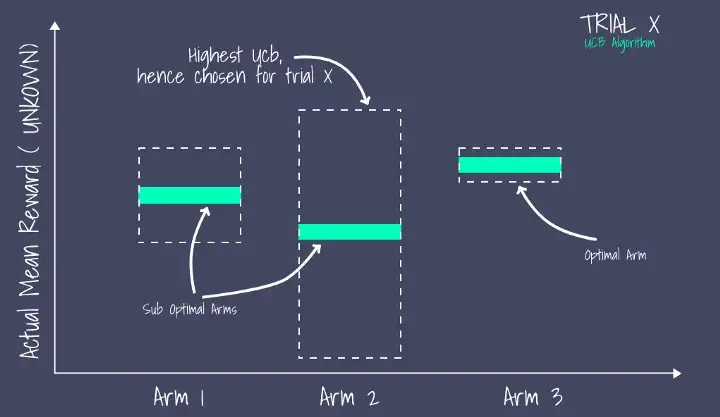
\includegraphics[scale=0.58]{Images/Learning_compensations/linucb.jpg}
    \caption{LinUCB algorithm for choosing the best arm \cite{recommender2020}.}
    \label{fig:linucb}
\end{figure}

Algorithm \ref{alg:linucb} shows the LinUCB algorithm. Let $d$ be the number of variables of the context $x_{t,a}$ (state). In our experiments, $d=3$. $A_a$ and $b_a$ are the variables used in ridge regression. This regression tries to find the correlation between state and reward. Lines 2-5 initialize both $A_a$ and $b_a$. This initialization makes all arms (actions) start with a very high UCB, forcing each arm to be chosen at least once. So, for each step t (line 6), it calculates the UCB for every arm (lines 7-10). To do so, line 8 calculates the ridge regression ($\hat{\theta_a}$), and line 9 applies it to find the UCB. The UCB $\rho_{t, a}$ is calculated by $\rho_{t, a} \leftarrow \hat{\theta_a}^\top x_{t,a} + \nu \sqrt{x_{t,a}^\top A_{a}^{-1} x_{t,a}}$, where the first part ($\hat{\theta_a}^\top x_{t,a}$) is the expected mean, and the second part ($\nu \sqrt{x_{t,a}^\top A_{a}^{-1} x_{t,a}}$) is the upper confidence bound. $\nu$ is a hyperparameter to indicate the importance of the standard deviation in the UCB. The higher $\nu$ is, the wider the confidence bounds become. So, a higher $\nu$ results in a higher emphasis placed on exploration instead of exploitation. We defined $\nu = 20$ after some experiments, with the best results with this value.

\IncMargin{1em}
\begin{algorithm}[!htb]
    \footnotesize
    \SetAlgoLined
    \Begin{
        \ForAll{a $\in A_t$ }{
            $A_a \leftarrow I_d$ (d-dimensional identity matrix)\;
            $b_a \leftarrow 0_{dx1}$ (d-dimensional zero vector)\;
        }        
        \For{t = 0, 1, 2, 3, ..., T}{
            \ForAll{a $\in A_t$ }{
                $\hat{\theta_a} \leftarrow A_{a}^{-1}b_a$\;
                $\rho_{t, a} \leftarrow \hat{\theta_a}^\top x_{t,a} + \nu \sqrt{x_{t,a}^\top A_{a}^{-1} x_{t,a}}$\;
            }
            Choose arm $a_t = \arg\max_{a \in A_t} \rho_{t, a}$, and observe a real-valued payoff $r_t$\; 
            $A_{a_{t}} \leftarrow A_{a_{t}} + x_{t,a_{t}} x_{t,a_{t}}^\top$\;
            $b_{a_{t}} \leftarrow b_{a_{t}} + r_t x_{t,a_{t}}$\;
        }
    }
    \caption{LinUCB algorithm \cite{li2010contextual}.}
    \label{alg:linucb}
\end{algorithm}
\DecMargin{1em}

Differently from Q-Learning, Contextual Multi-Armed Bandit does not need a discretization of the state. Therefore, we can use directly the state here, without modifications.

\section{Results Evaluation}

After presenting the algorithms, we apply them to the critical scenarios from the previous chapter. We have four different RL executions combining the RL algorithm and action: 

\begin{enumerate}
    \item \emph{Bandit + heuristic};
    \item \emph{Q-Learning + heuristic};
    \item \emph{Bandit + hour};
    \item \emph{Q-Learning + hour};
\end{enumerate}

These algorithms use the same scheduling from Chapter \ref{cha:power_compensations}, changing only in which step compensating. For each critical case, we run 200 iterations of each RL algorithm with the different reward types. The idea is to verify if the RL algorithms can learn by repeating the same inputs (workload and weather). Also, we want to verify if they can improve the number of finished jobs. We do not execute the average cases due to their complexity. They are 100 different cases, demanding high processing time for executing 200 iterations of each one. Again, the critical cases are:
\begin{enumerate}
    \item \emph{Critical 1}: Profile best-case and workload in the beginning;
    \item \emph{Critical 2}: Profile best-case and workload in the end;
    \item \emph{Critical 3}: Profile worst-case and workload in the beginning;
    \item \emph{Critical 4}: Profile worst-case and workload in the end;
\end{enumerate}

The results from the baselines and compensation policies (\emph{Last}, \emph{Next}, \emph{Peak}, and \emph{Workload}) are the same results from the previous chapter. We compare them with the new results from Reinforcement Learning. The results of the random algorithms are an average of 200 iterations.

\subsection{Started Jobs Reward}

Starting with the reward Started Jobs, we present the results in the four critical cases in Figures \ref{fig:started_reward_results_critical_1}, \ref{fig:started_reward_results_critical_2}, \ref{fig:started_reward_results_critical_3}, and \ref{fig:started_reward_results_critical_4}. Each figure shows 5 graphs. The first two on top are the graphs about the finished jobs. The two graphs in the middle are the battery level and wasted energy. These are the same graphs from the previous chapter. The last graph is the reward evolution over the 200 iterations. The reward is calculated by summing all rewards from the different actions inside the iteration.

\begin{figure}[!htb]
    \centering
    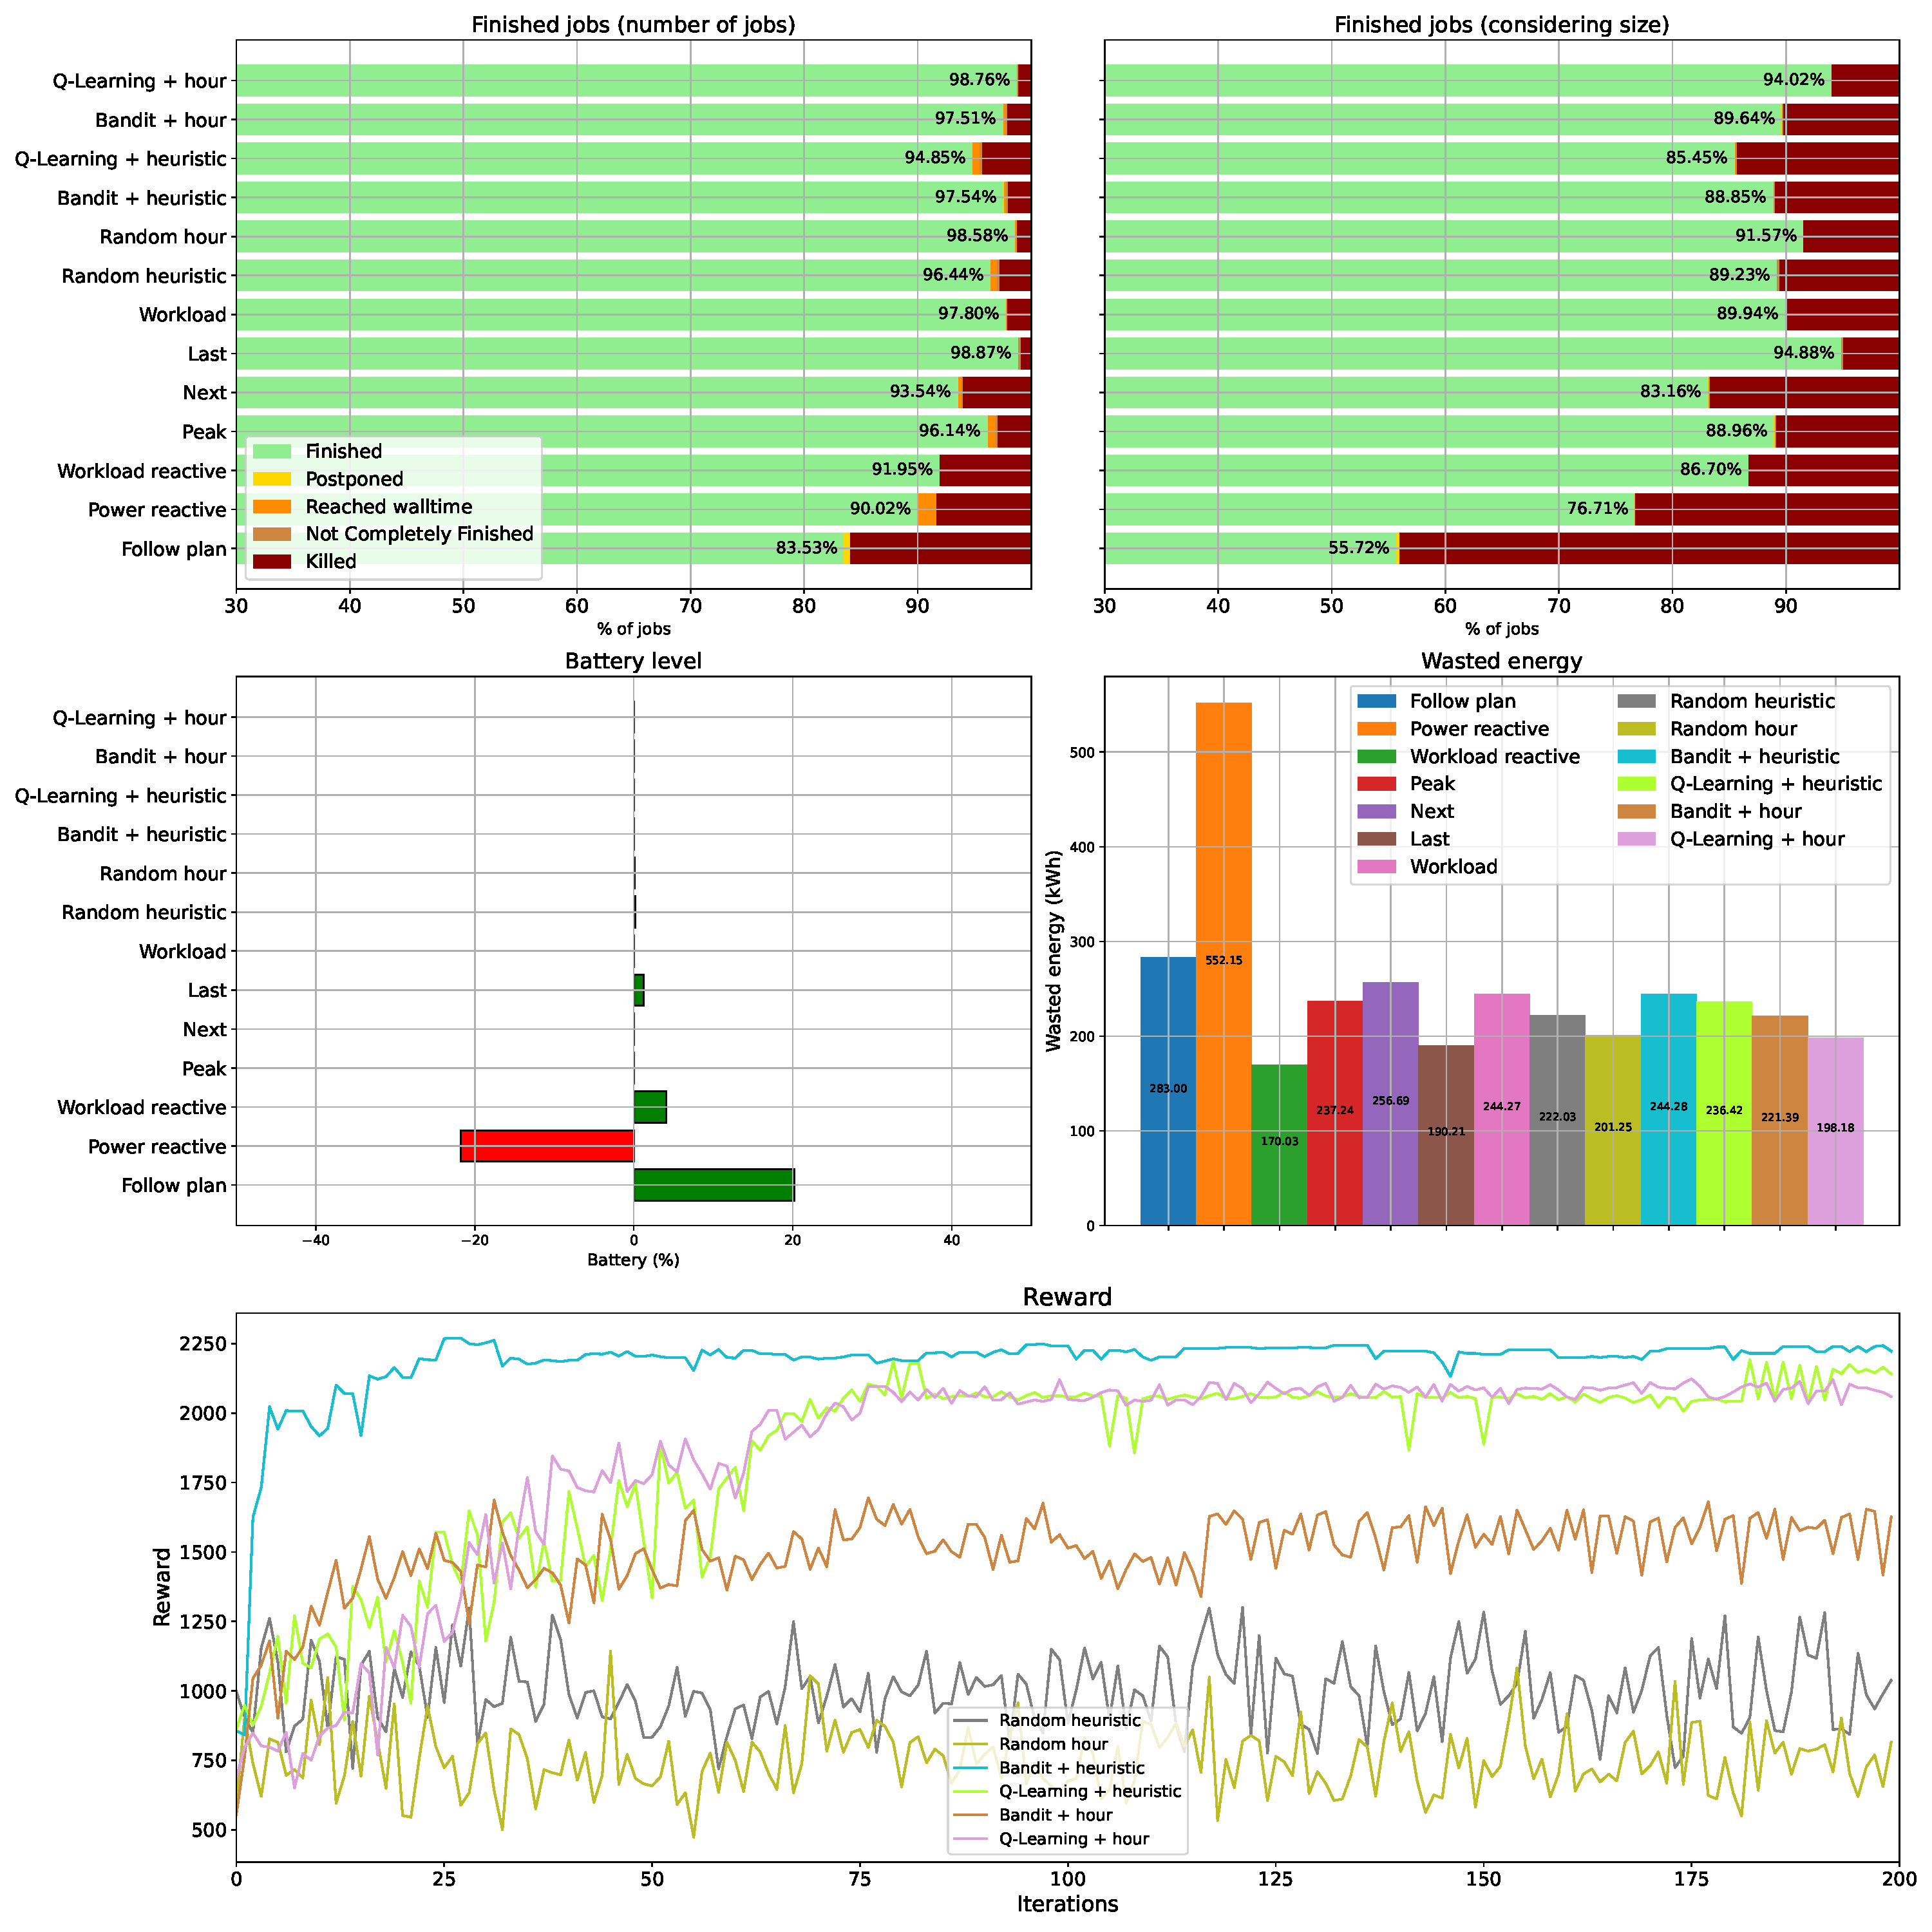
\includegraphics[scale=0.29]{Images/Learning_compensations/reward_started_profile_best_workload_1_with_noise_state_delta.pdf}
    \caption{Results of reward started jobs in critical case 1.}
    \label{fig:started_reward_results_critical_1}
\end{figure}

\begin{figure}[!htb]
    \centering
    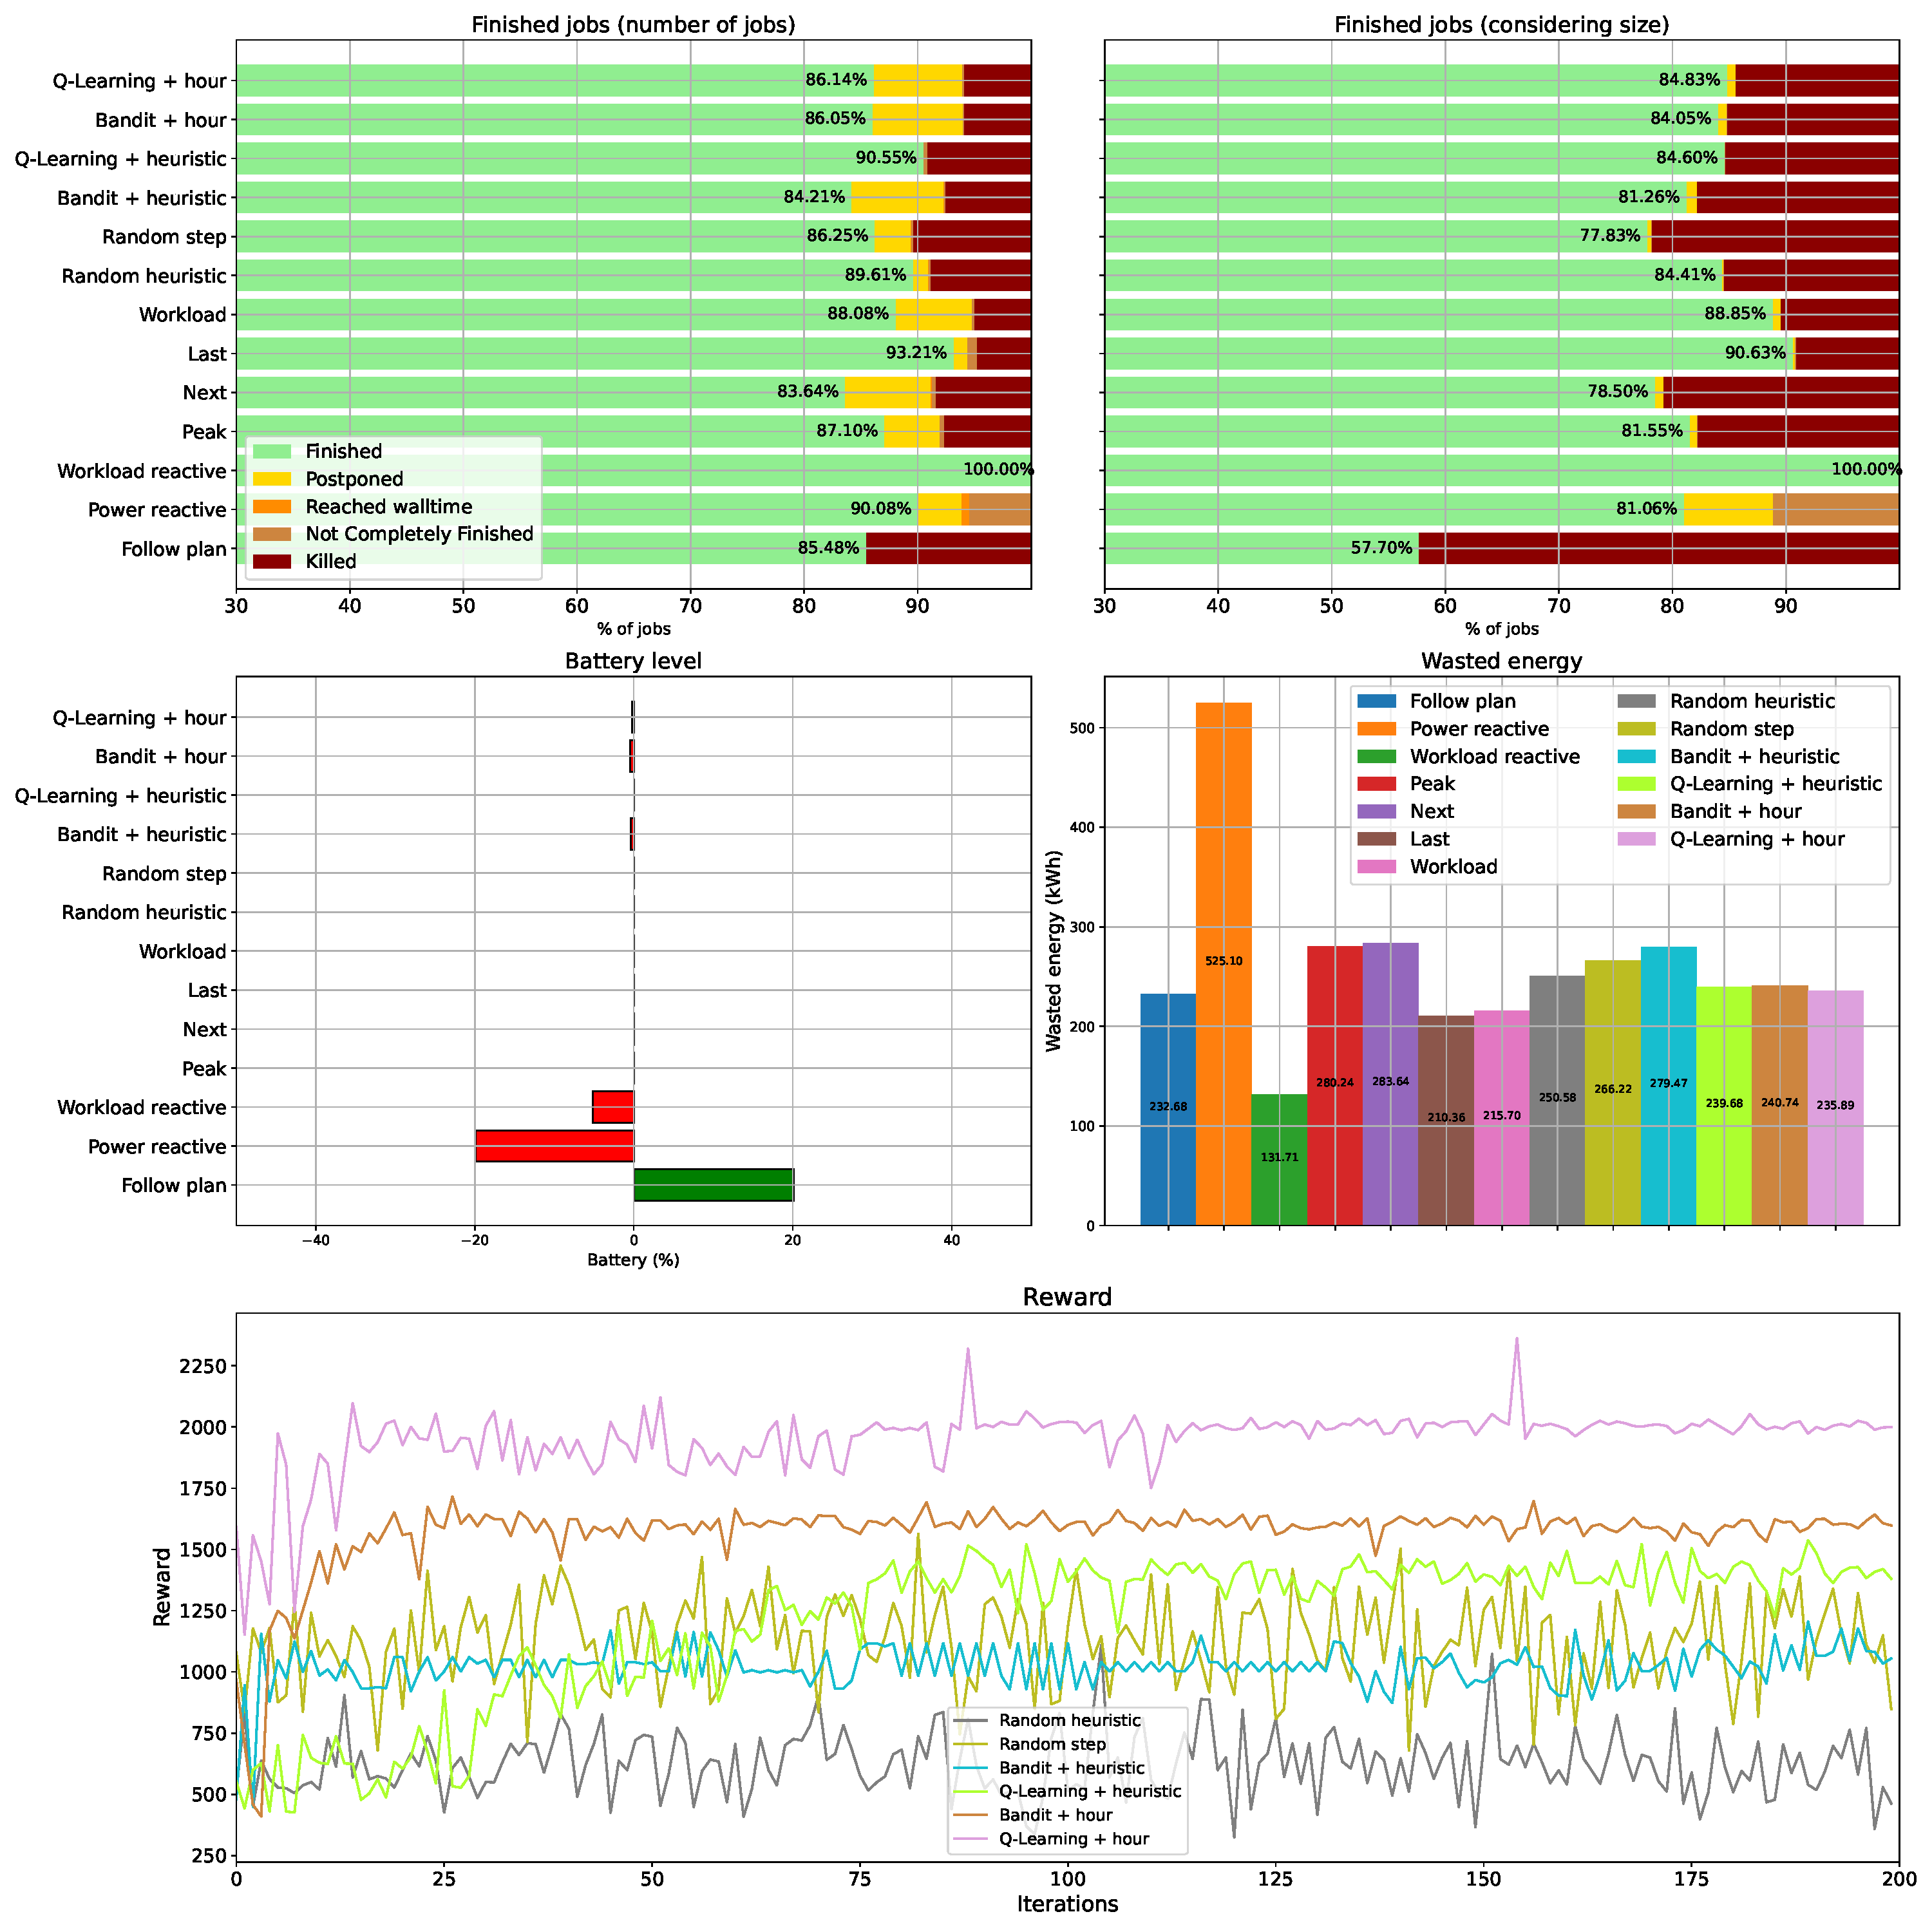
\includegraphics[scale=0.29]{Images/Learning_compensations/reward_started_profile_best_workload_2_with_noise_state_delta.pdf}
    \caption{Results of reward started jobs in critical case 2.}
    \label{fig:started_reward_results_critical_2}
\end{figure}

\begin{figure}[!htb]
    \centering
    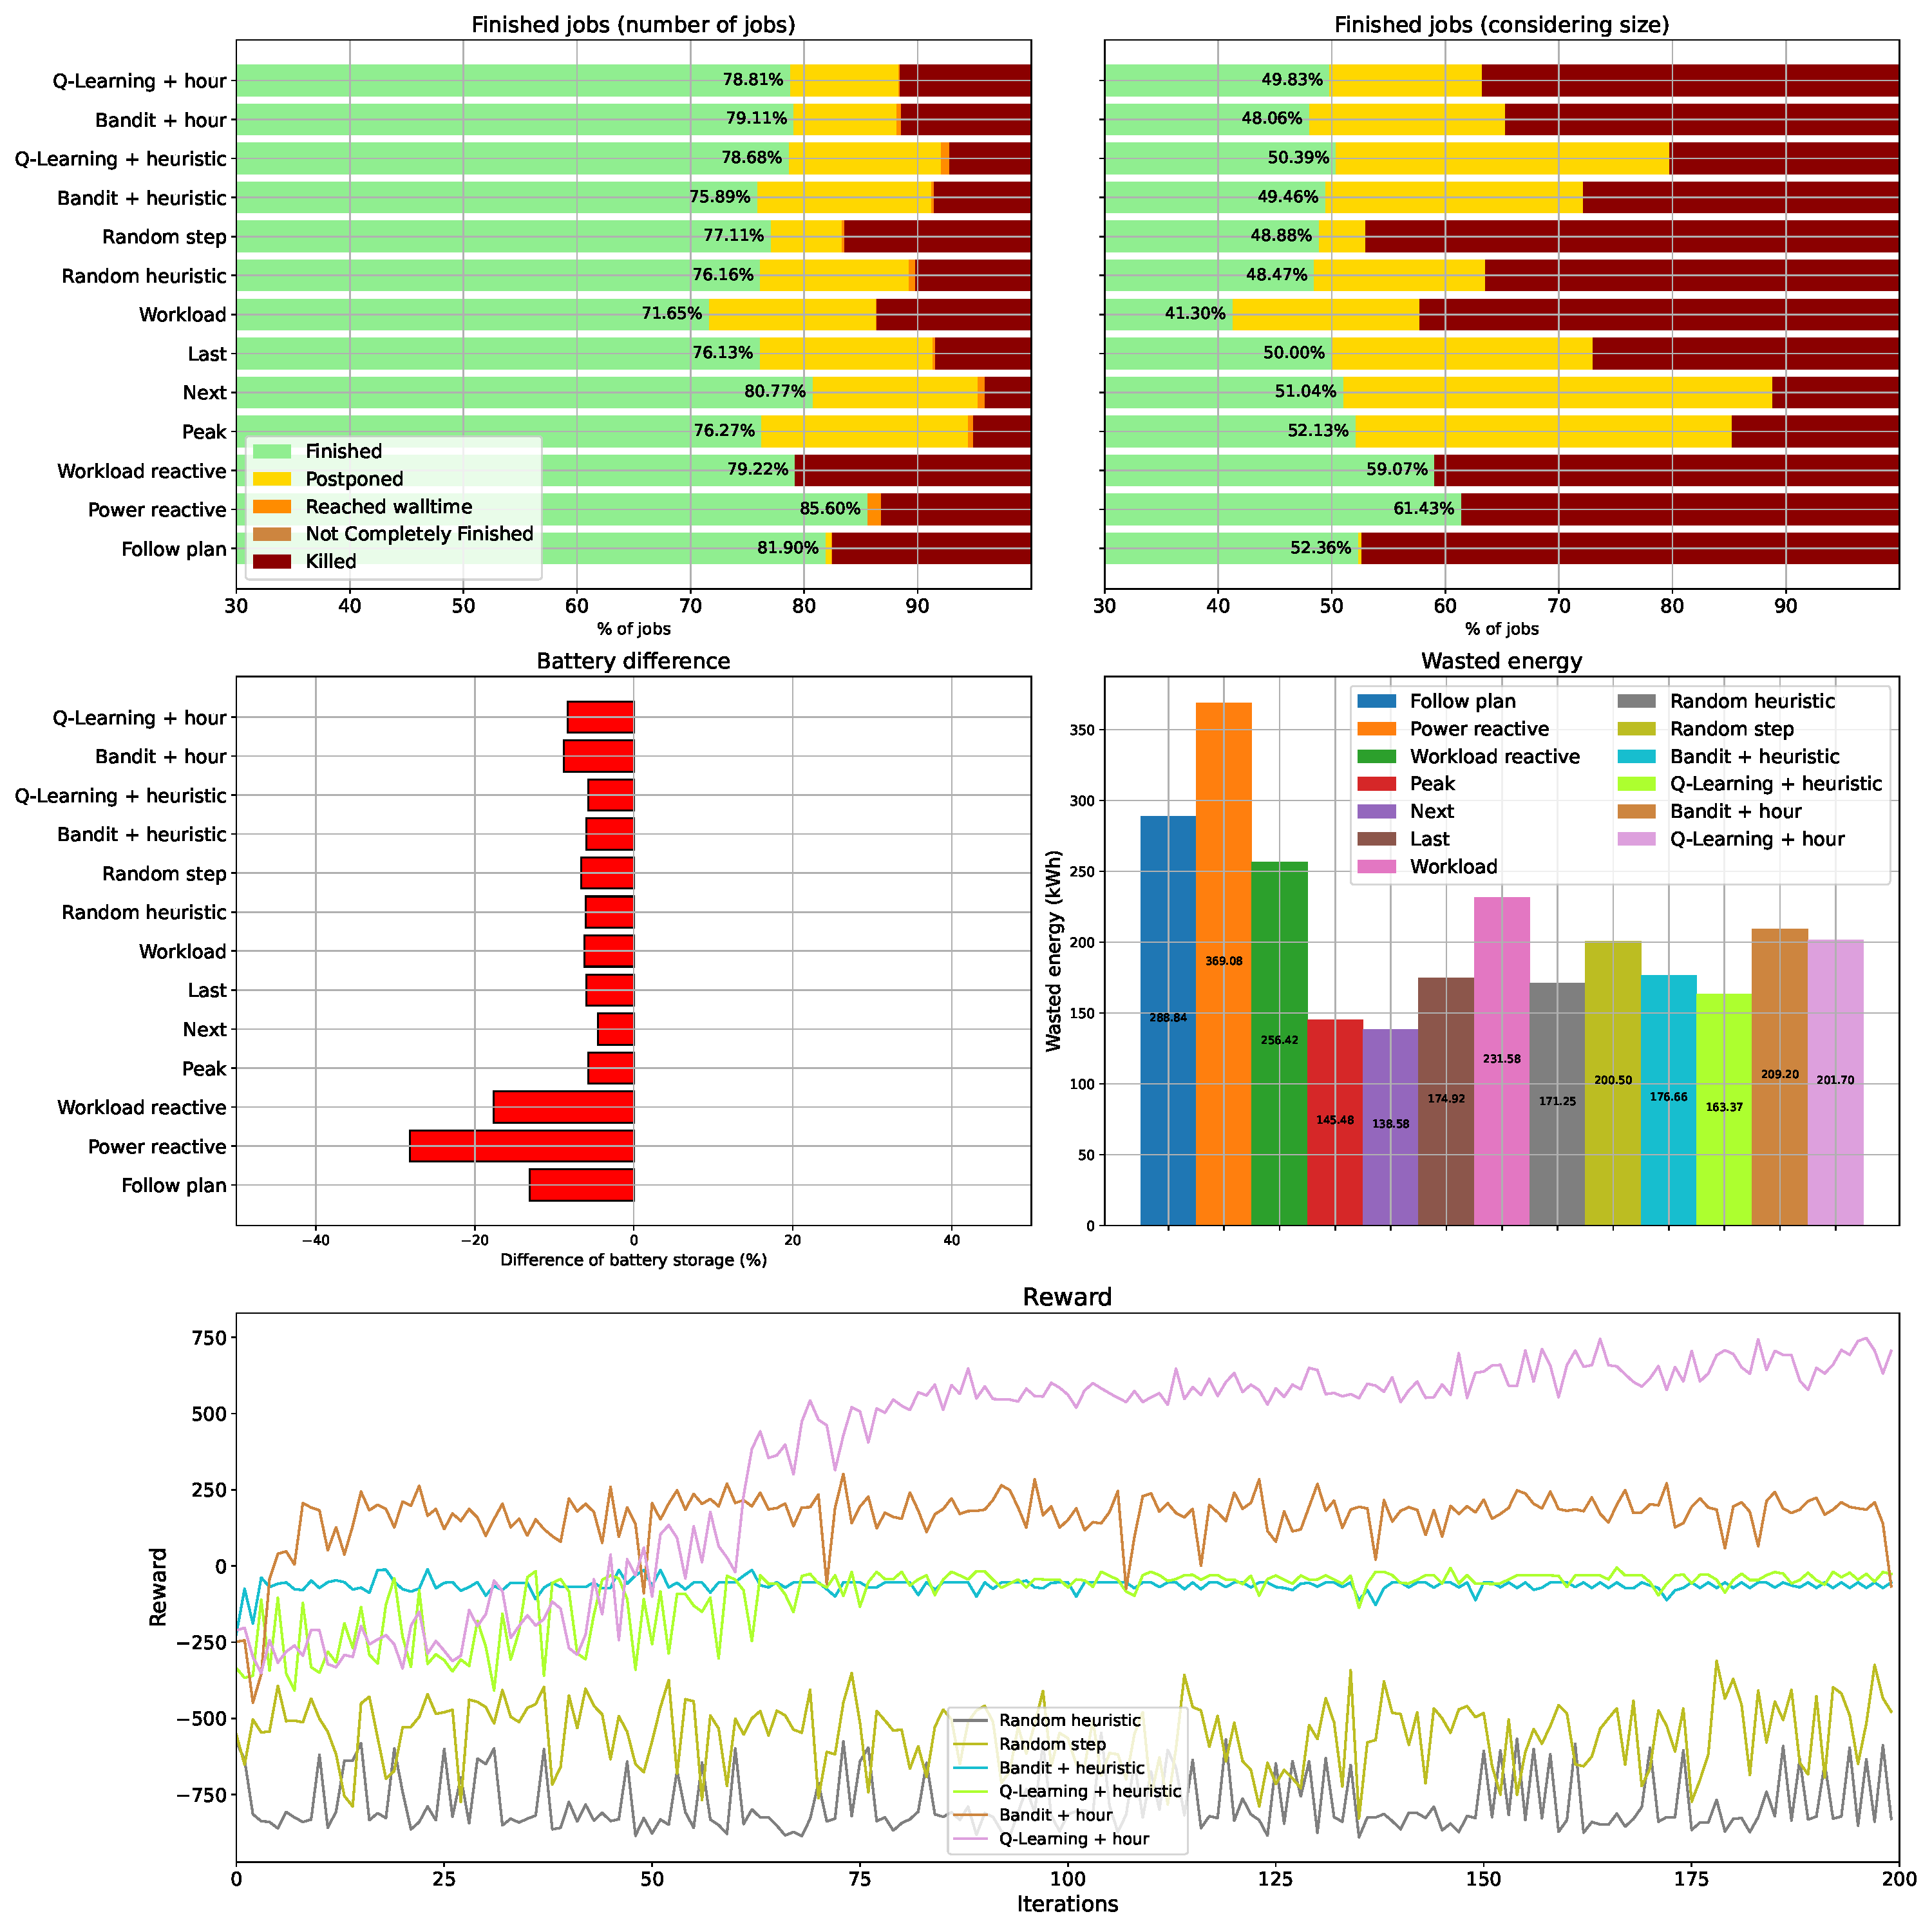
\includegraphics[scale=0.29]{Images/Learning_compensations/reward_started_profile_worst_workload_1_with_noise_state_delta.pdf}
    \caption{Results of reward started jobs in critical case 3.}
    \label{fig:started_reward_results_critical_3}
\end{figure}

\begin{figure}[!htb]
    \centering
    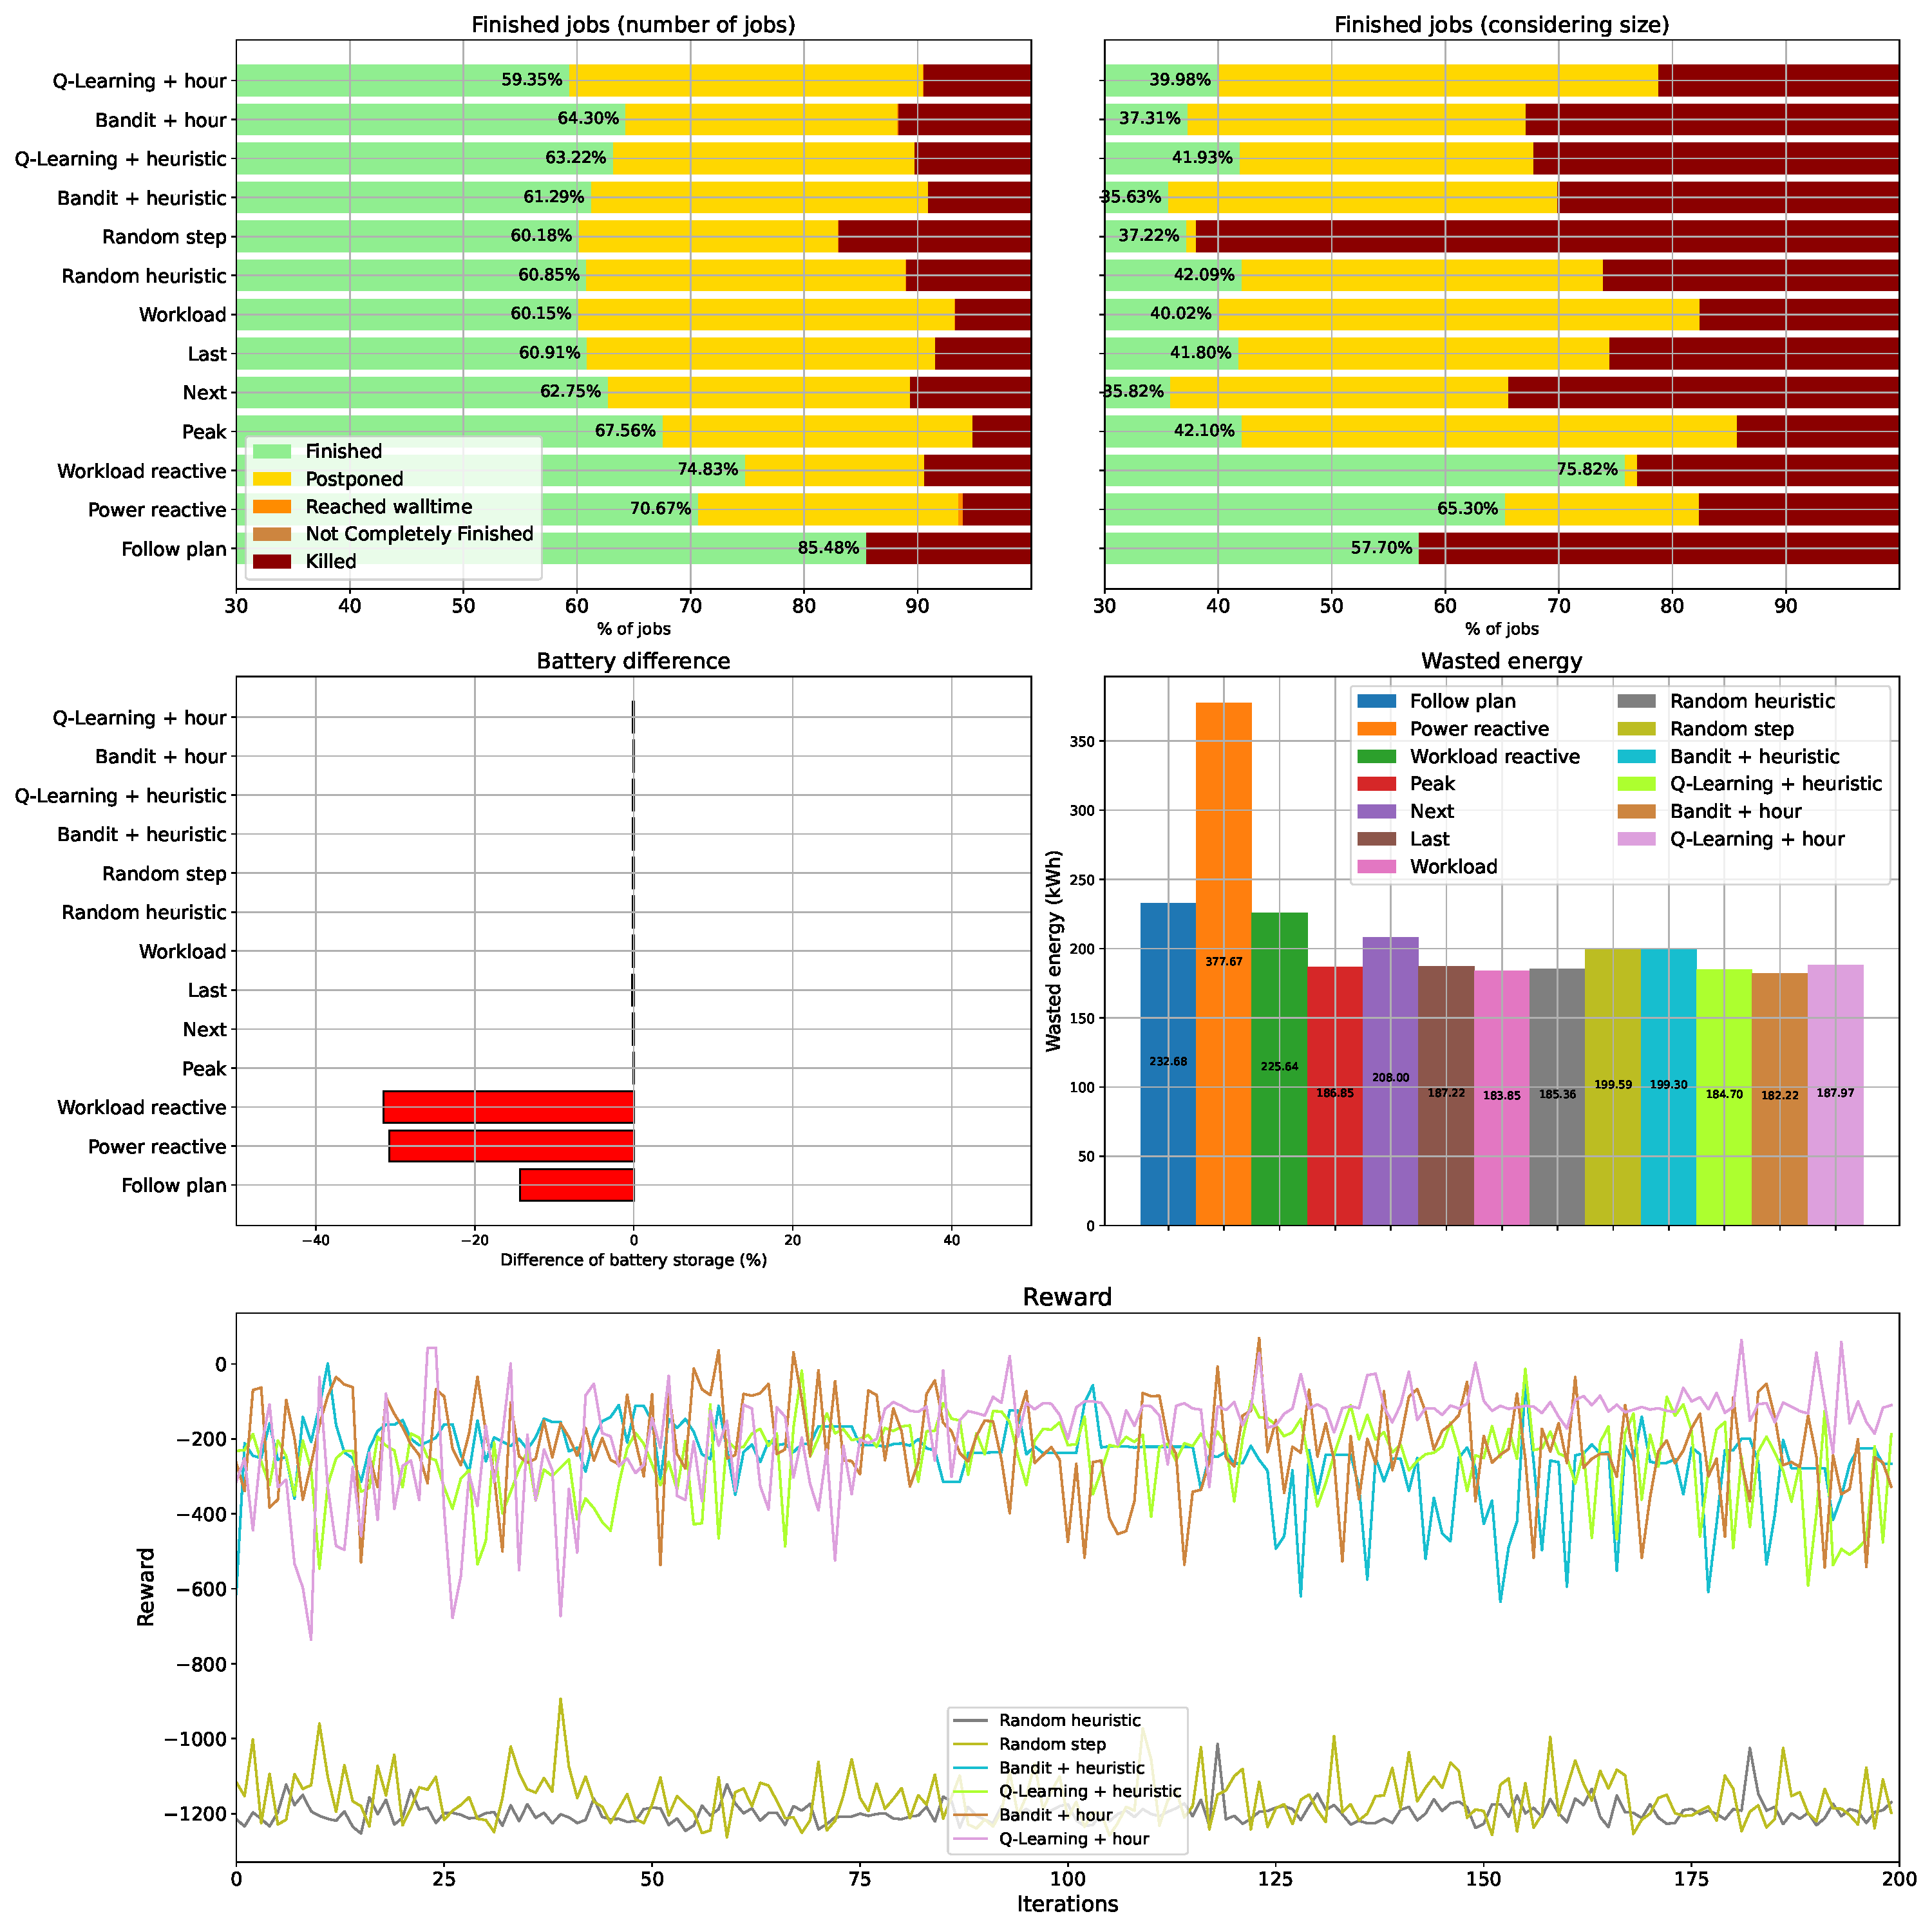
\includegraphics[scale=0.29]{Images/Learning_compensations/reward_started_profile_worst_workload_2_with_noise_state_delta.pdf}
    \caption{Results of reward started jobs in critical case 4.}
    \label{fig:started_reward_results_critical_4}
\end{figure}

Figure \ref{fig:started_reward_results_critical_1} shows that in critical case 1, all RL improved their reward over time. They started with similar rewards to random executions. However, at the end of 200 iterations, they improved the reward. This result shows us that the algorithms are finding the decisions which give higher rewards. Considering the reward, the best algorithms are, in order, \emph{Bandit + heuristic}, \emph{Q-Learning + heuristic}, \emph{Q-Learning + hour}, and \emph{Bandit + hour}. However, considering the finished jobs in number (first graph), the results indicate \emph{Q-Learning + hour} as the best one, with both Bandit algorithms as the second one with similar results. So, even with a big difference in the reward of both bandits, they have similar results. This result shows a problem in this reward, where just starting jobs does not guarantee they will finish. Also, the best RL result is still worst than the \emph{Last} policy in the finished jobs metric (both in number and size). Considering the Battery level, all RL algorithms have the same results. Finally, both Bandit and Q-Learning algorithms expend more energy than \emph{Last} policy in this case.

The results of critical case 2 in Figure \ref{fig:started_reward_results_critical_2} show that only the RL algorithms using the action of the hour to compensate could improve the reward. Among the two RL algorithms using hour, \emph{Q-Learning + hour} has a better reward than \emph{Bandit + hour}, but considering the number of finished jobs, \emph{Bandit + hour} is better than \emph{Q-Learning + hour}. Considering the size, \emph{Bandit + hour} is worst than \emph{Q-Learning + hour}. Comparing these results with the policies, \emph{Bandit + hour} is better than \emph{Last} policy (the best policy) in the number of finished jobs. However, \emph{Bandit + hour} kills more jobs and uses more battery than \emph{Last}. Considering the size, \emph{Last} is still better. All RL algorithms wasted more energy than the \emph{Last} policy in this case.

Starting the cases with less energy, Figure \ref{fig:started_reward_results_critical_3} illustrates the results of critical case 3. Here, again, all RL algorithms have higher rewards than both random algorithms. Again, the \emph{Q-Learning + hour} and \emph{Bandit + hour} have the best results among the RL algorithms. \emph{Bandit + hour} has a lower reward, but a higher number of jobs finished. \emph{Bandit + hour} has similar finished jobs than \emph{Next} in number and \emph{Peak} in size (both policies are the best ones in each metric). However, \emph{Bandit + hour} kills more jobs than both policies. Considering the battery level, \emph{Q-Learning + hour} and \emph{Bandit + hour} use slightly more battery than the other policies. But, they are all below the baselines. Finally, the wasted energy results of the RL algorithms are higher than the \emph{Peak} and \emph{Next} policies.

Figure \ref{fig:started_reward_results_critical_4} present the last scenario, critical case 4. All RL algorithms have higher rewards than random heuristics. \emph{Bandit + hour} has the higher number of finished jobs with less than 10\% of killed jobs (in number). It has the highest finished jobs compared to the policies. However, it kills more jobs than some policies (e.g., \emph{Peak}). Also, it has almost 14\% of battery deficit, almost the same deficit as \emph{Follow plan}. Again, \emph{Q-Learning + hour} has the higher reward but with several killed jobs and not the higher finished jobs. The RL algorithms wasted more energy than \emph{Workload} (the best policy).

Consolidating the results of Started Jobs Reward, it is possible to notice that \emph{Q-Learning + hour} and \emph{Bandit + hour} improved the reward after 200 iterations. Usually, the reward from these cases has a distance from the random rewards after 200 iterations. This result indicates that the RL learning algorithms are learning the policies to choose the actions which give a high reward. However, having a high reward does not result in a good global result (mainly finished/killed jobs). \emph{Bandit + hour} has a higher number of finished jobs than the policies in two cases (critical cases 2 and 4) but with higher killed jobs than the policies. This reward reinforces the actions which put more energy into steps that start more jobs. However, starting jobs does not mean that they will finish. So, it can start several jobs, but kill a lot also. Aiming to solve this problem (starting some jobs but not finishing them), we proposed the next reward.

\subsection{Finished Jobs Reward}

The next reward aims to solve the problem of starting jobs and not finishing them. So, this reward reinforces the actions that help to finish more jobs. Figures \ref{fig:touched_reward_results_critical_1}, \ref{fig:touched_reward_results_critical_2}, \ref{fig:touched_reward_results_critical_3}, and \ref{fig:touched_reward_results_critical_4} present the results of this reward.

\begin{figure}[!htb]
    \centering
    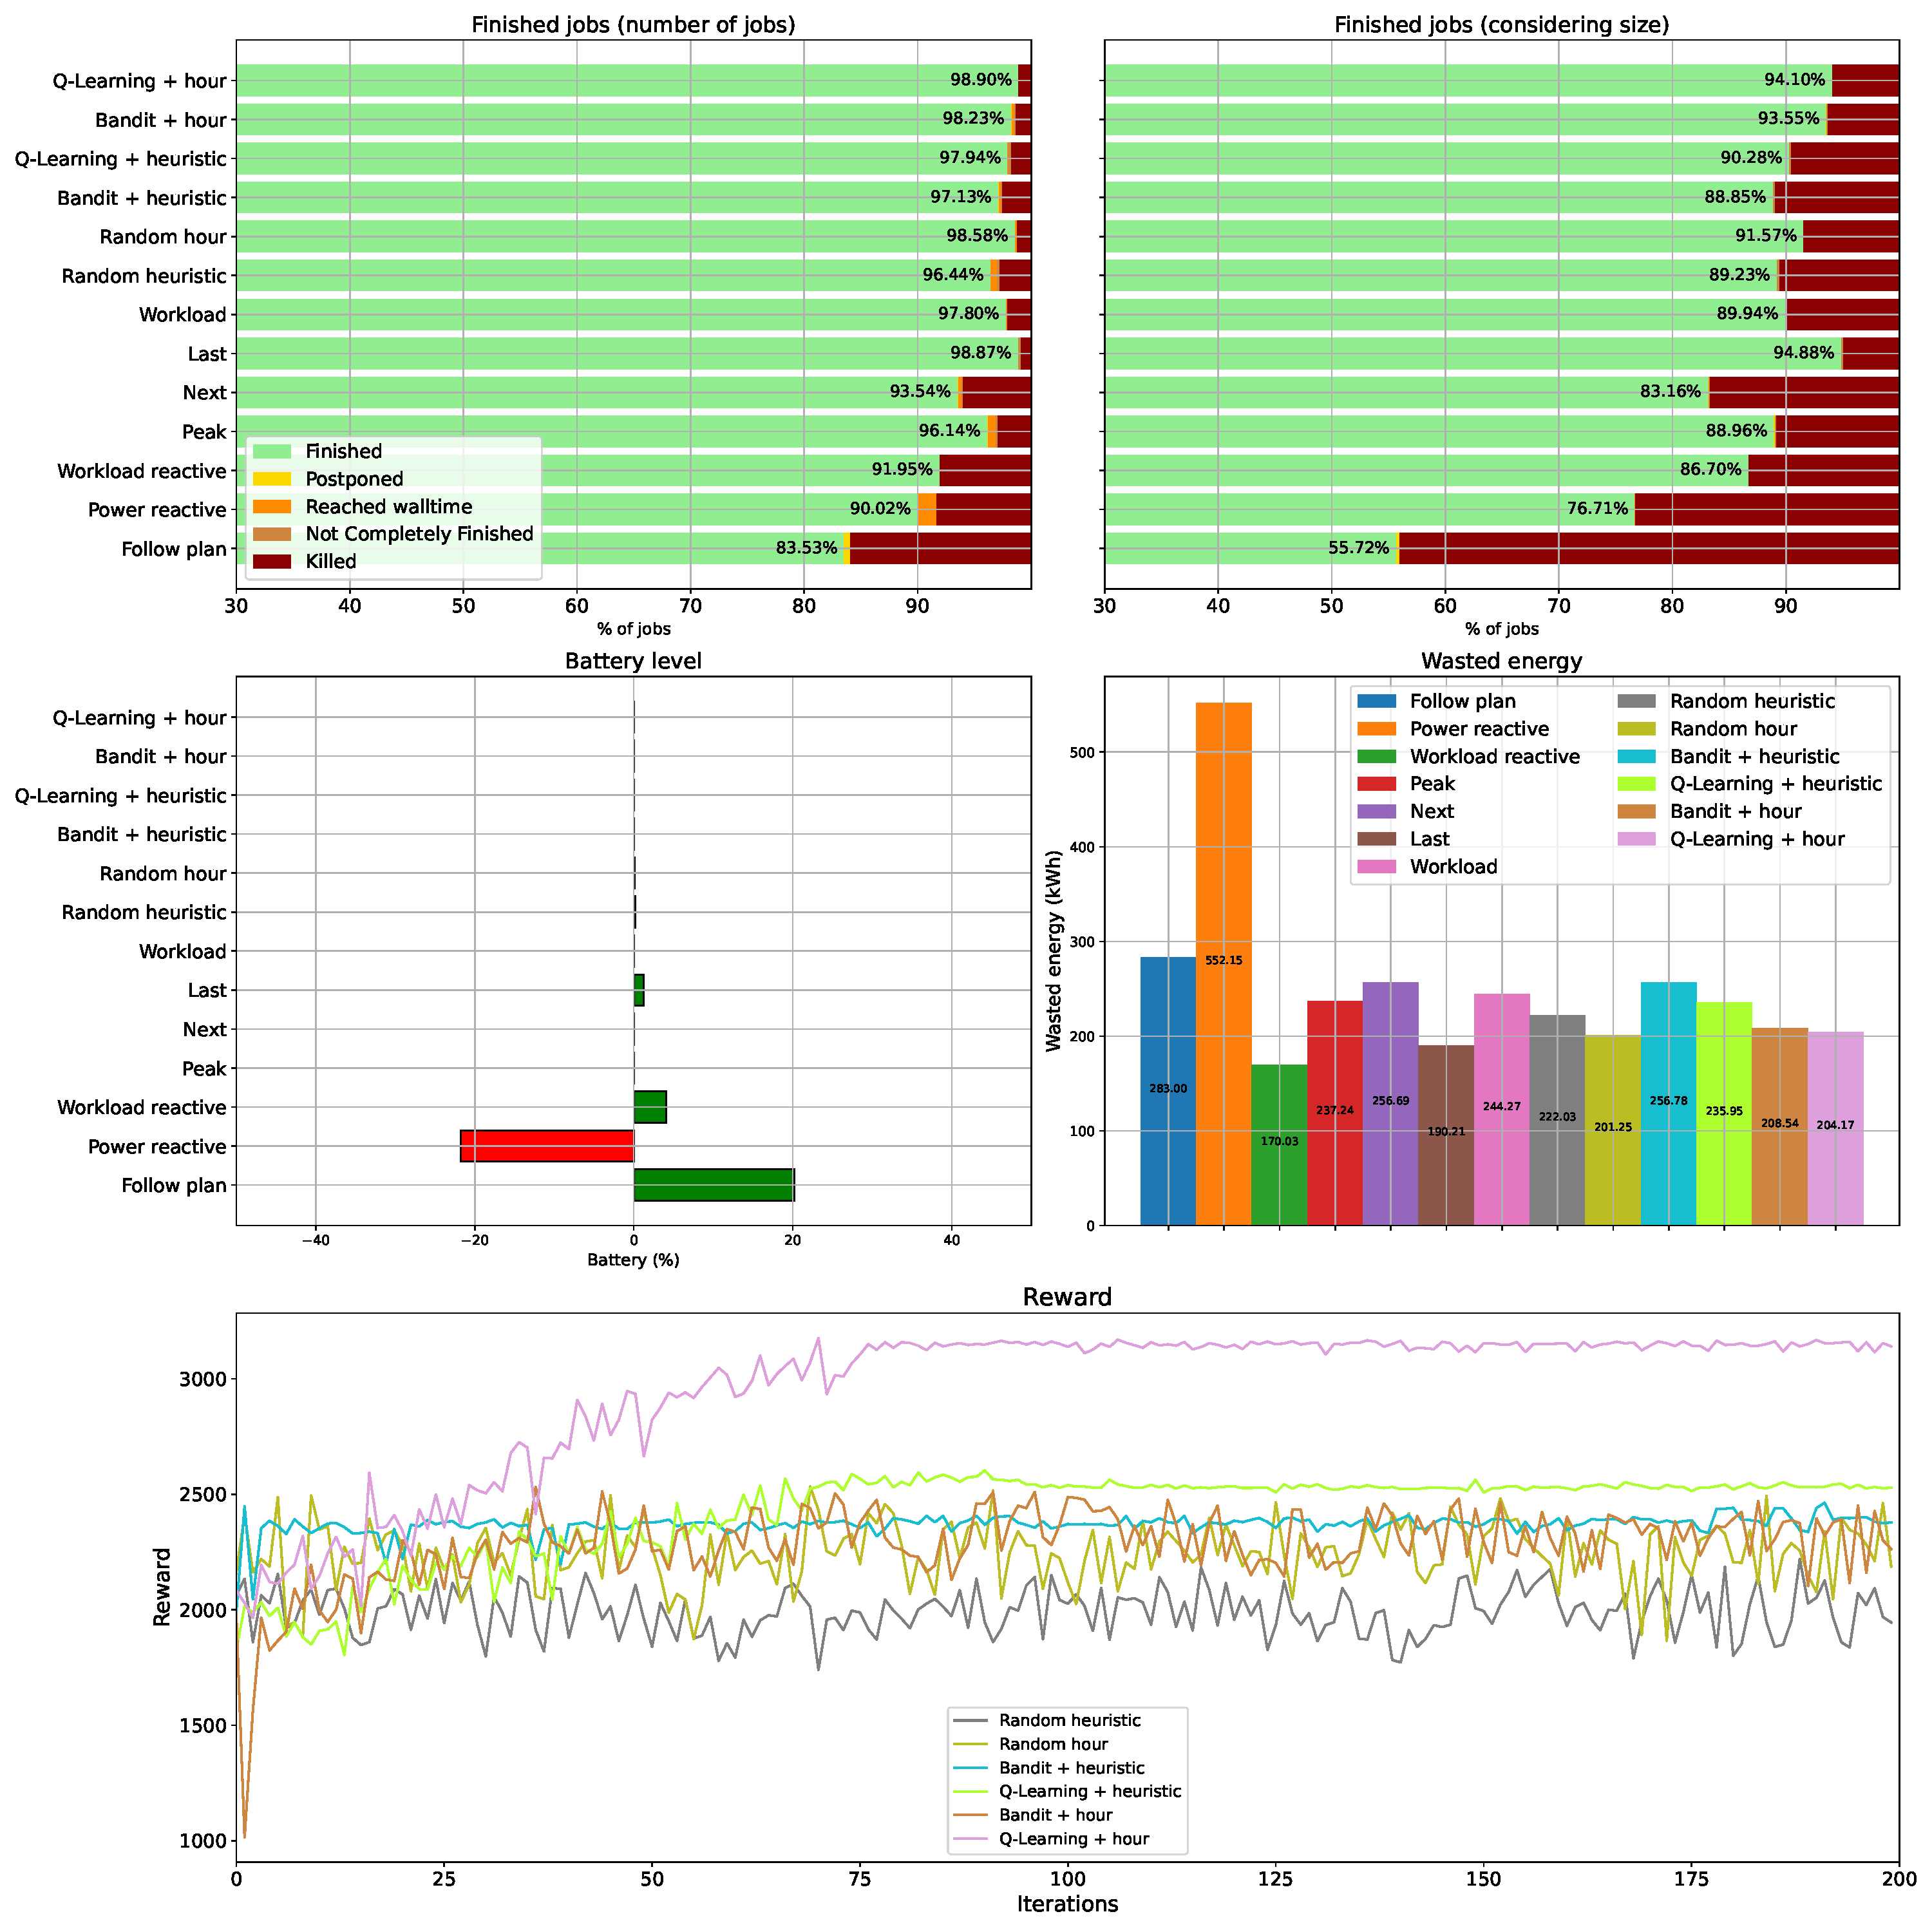
\includegraphics[scale=0.29]{Images/Learning_compensations/reward_finished_touched_profile_best_workload_1_with_noise_state_delta.pdf}
    \caption{Results of finished jobs reward in critical case 1.}
    \label{fig:touched_reward_results_critical_1}
\end{figure}

Starting with critical case 1, Figure \ref{fig:touched_reward_results_critical_1} illustrates the results. Now, the highest reward is from \emph{Q-Learning + hour} which also has the higher number of jobs finished and size among the RL algorithms. However, the second best reward is \emph{Q-Learning + heuristic} which is worst than \emph{Bandit + hour}. So, we still have some problems with the reward. Figure \ref{fig:reward_from_jobs_critical_1} highlights the problem of this reward. This figure illustrates in red the total finished jobs and in blue the finished jobs included in the reward over the iterations. It is possible to notice that the reward's improvement of \emph{Q-Learning + heuristic} is not linked to more jobs finished, but because it includes more finished jobs in its reward. So, it puts energy into steps with more finished jobs just to receive the reward of them. \emph{Bandit + hour} "touched" fewer jobs, even finishing quite the same number of the jobs. Another point is that they do not increase the number of jobs finished, comparing the first iterations to the last ones, having constant finished jobs. Therefore, they do not improve the finished jobs in this execution.

\begin{figure}[!htb]
    \centering
    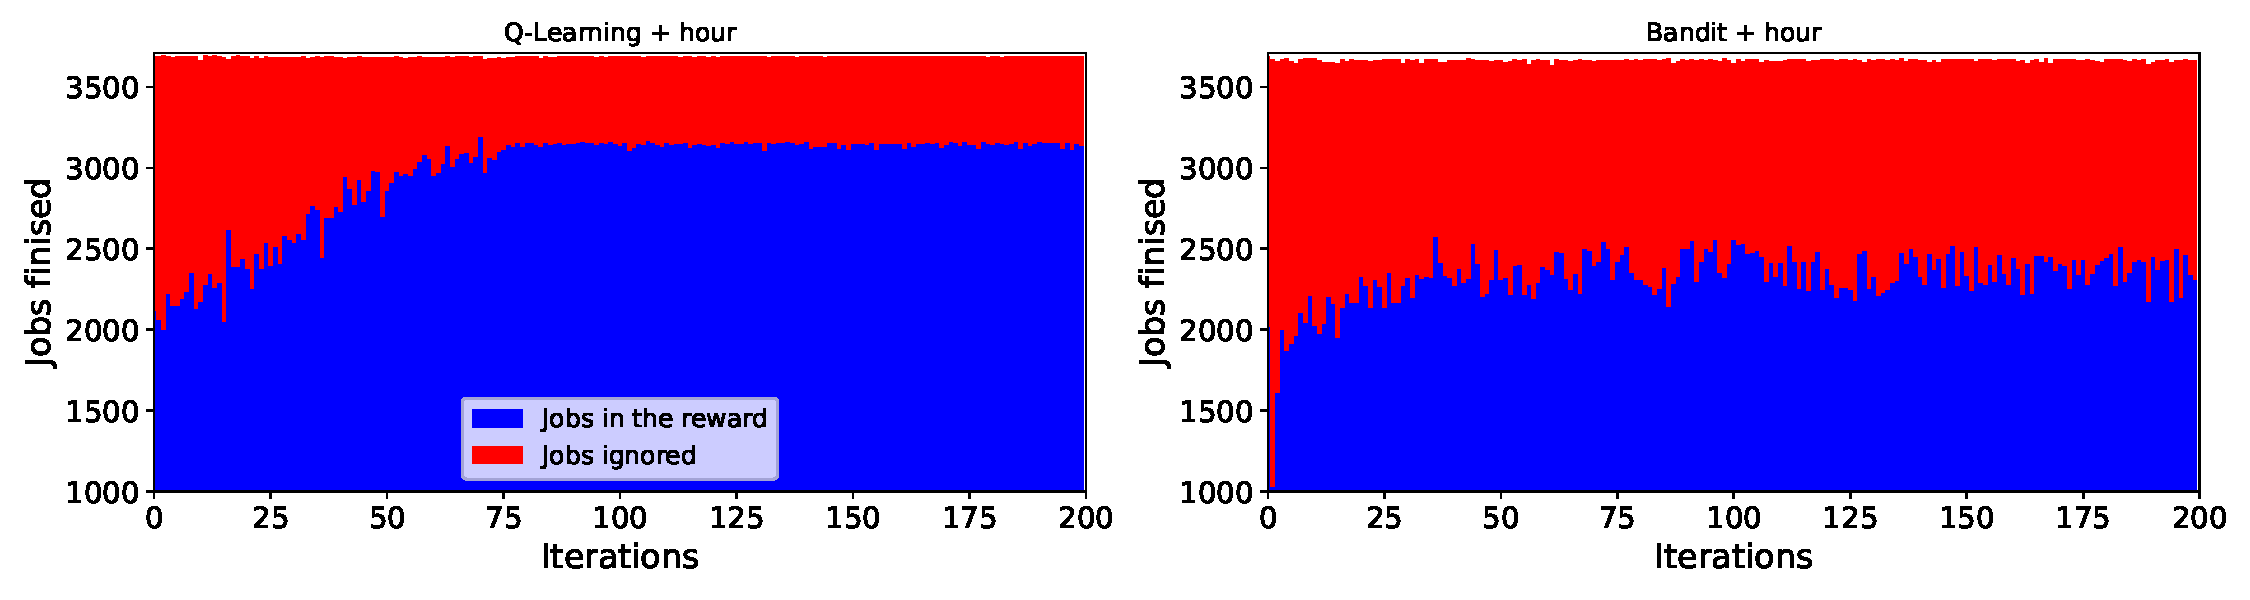
\includegraphics[scale=0.38]{Images/Learning_compensations/ignored_jobs_touched_scenario_1.pdf}
    \caption{Total finished jobs (in red) and jobs included in the reward (in blue).}
    \label{fig:reward_from_jobs_critical_1}
\end{figure}

\begin{figure}[!htb]
    \centering
    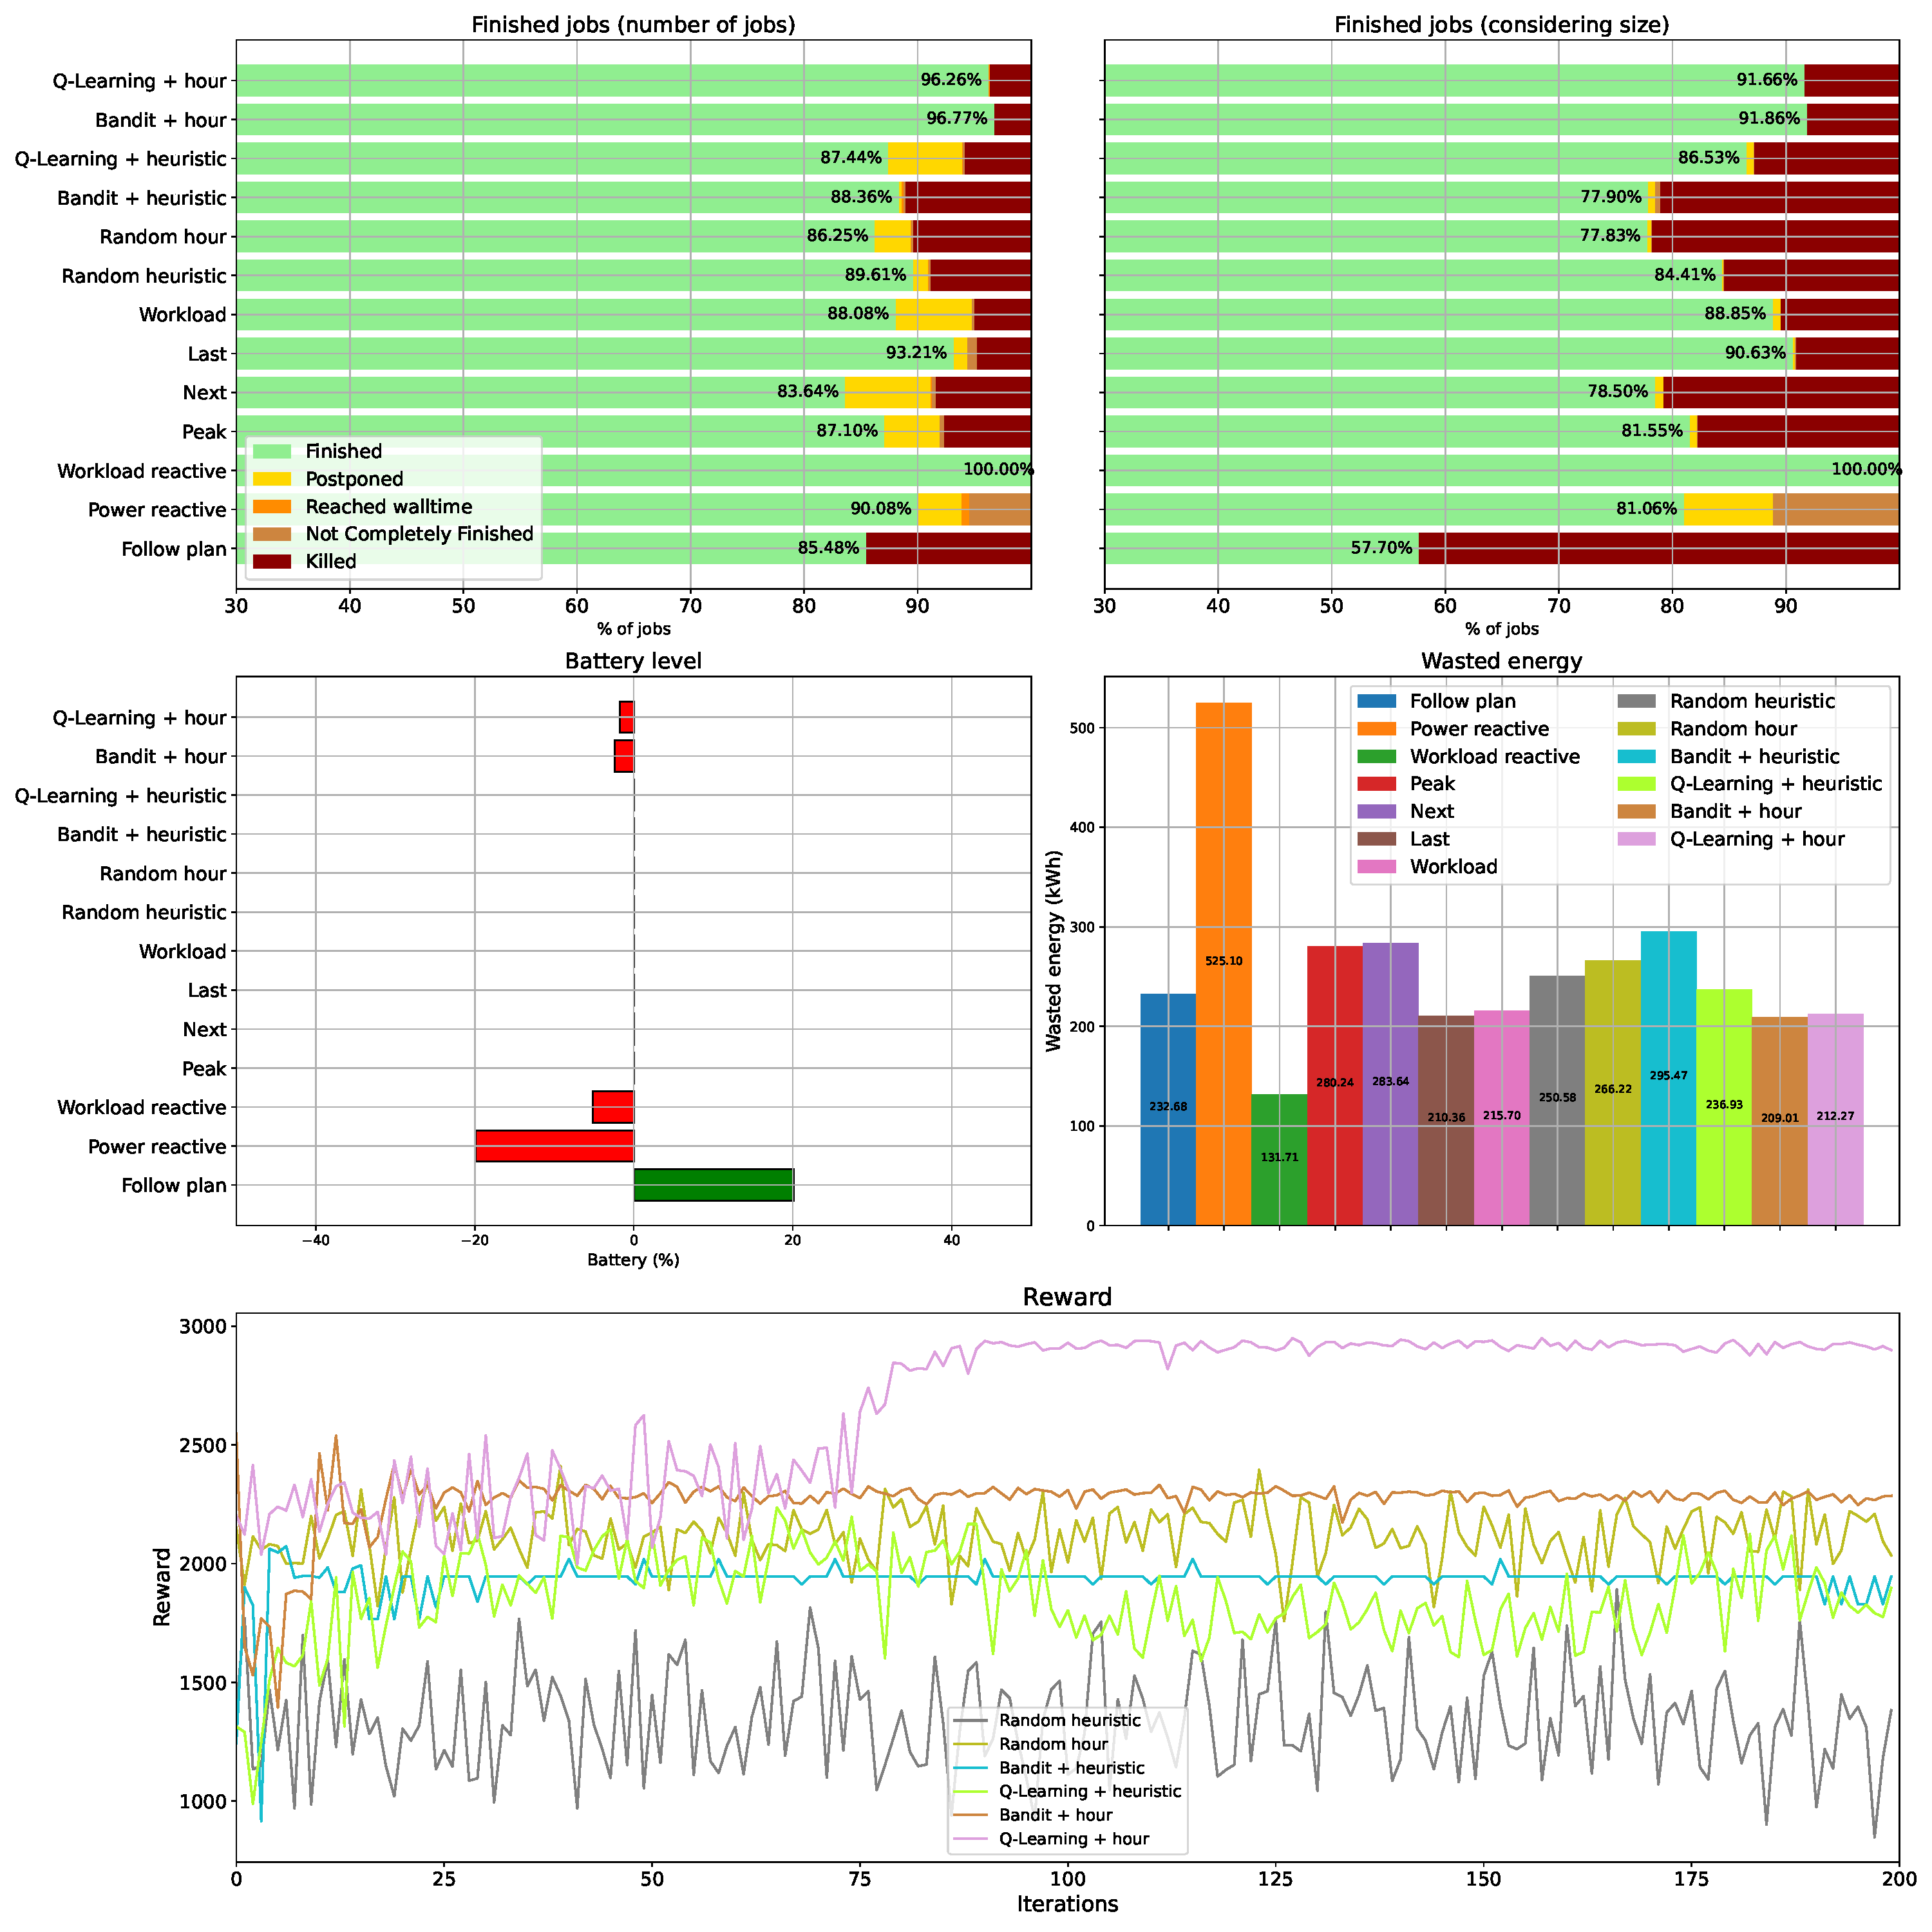
\includegraphics[scale=0.29]{Images/Learning_compensations/reward_finished_touched_profile_best_workload_2_with_noise_state_delta.pdf}
    \caption{Results of finished jobs reward in critical case 2.}
    \label{fig:touched_reward_results_critical_2}
\end{figure}

\begin{figure}[!htb]
    \centering
    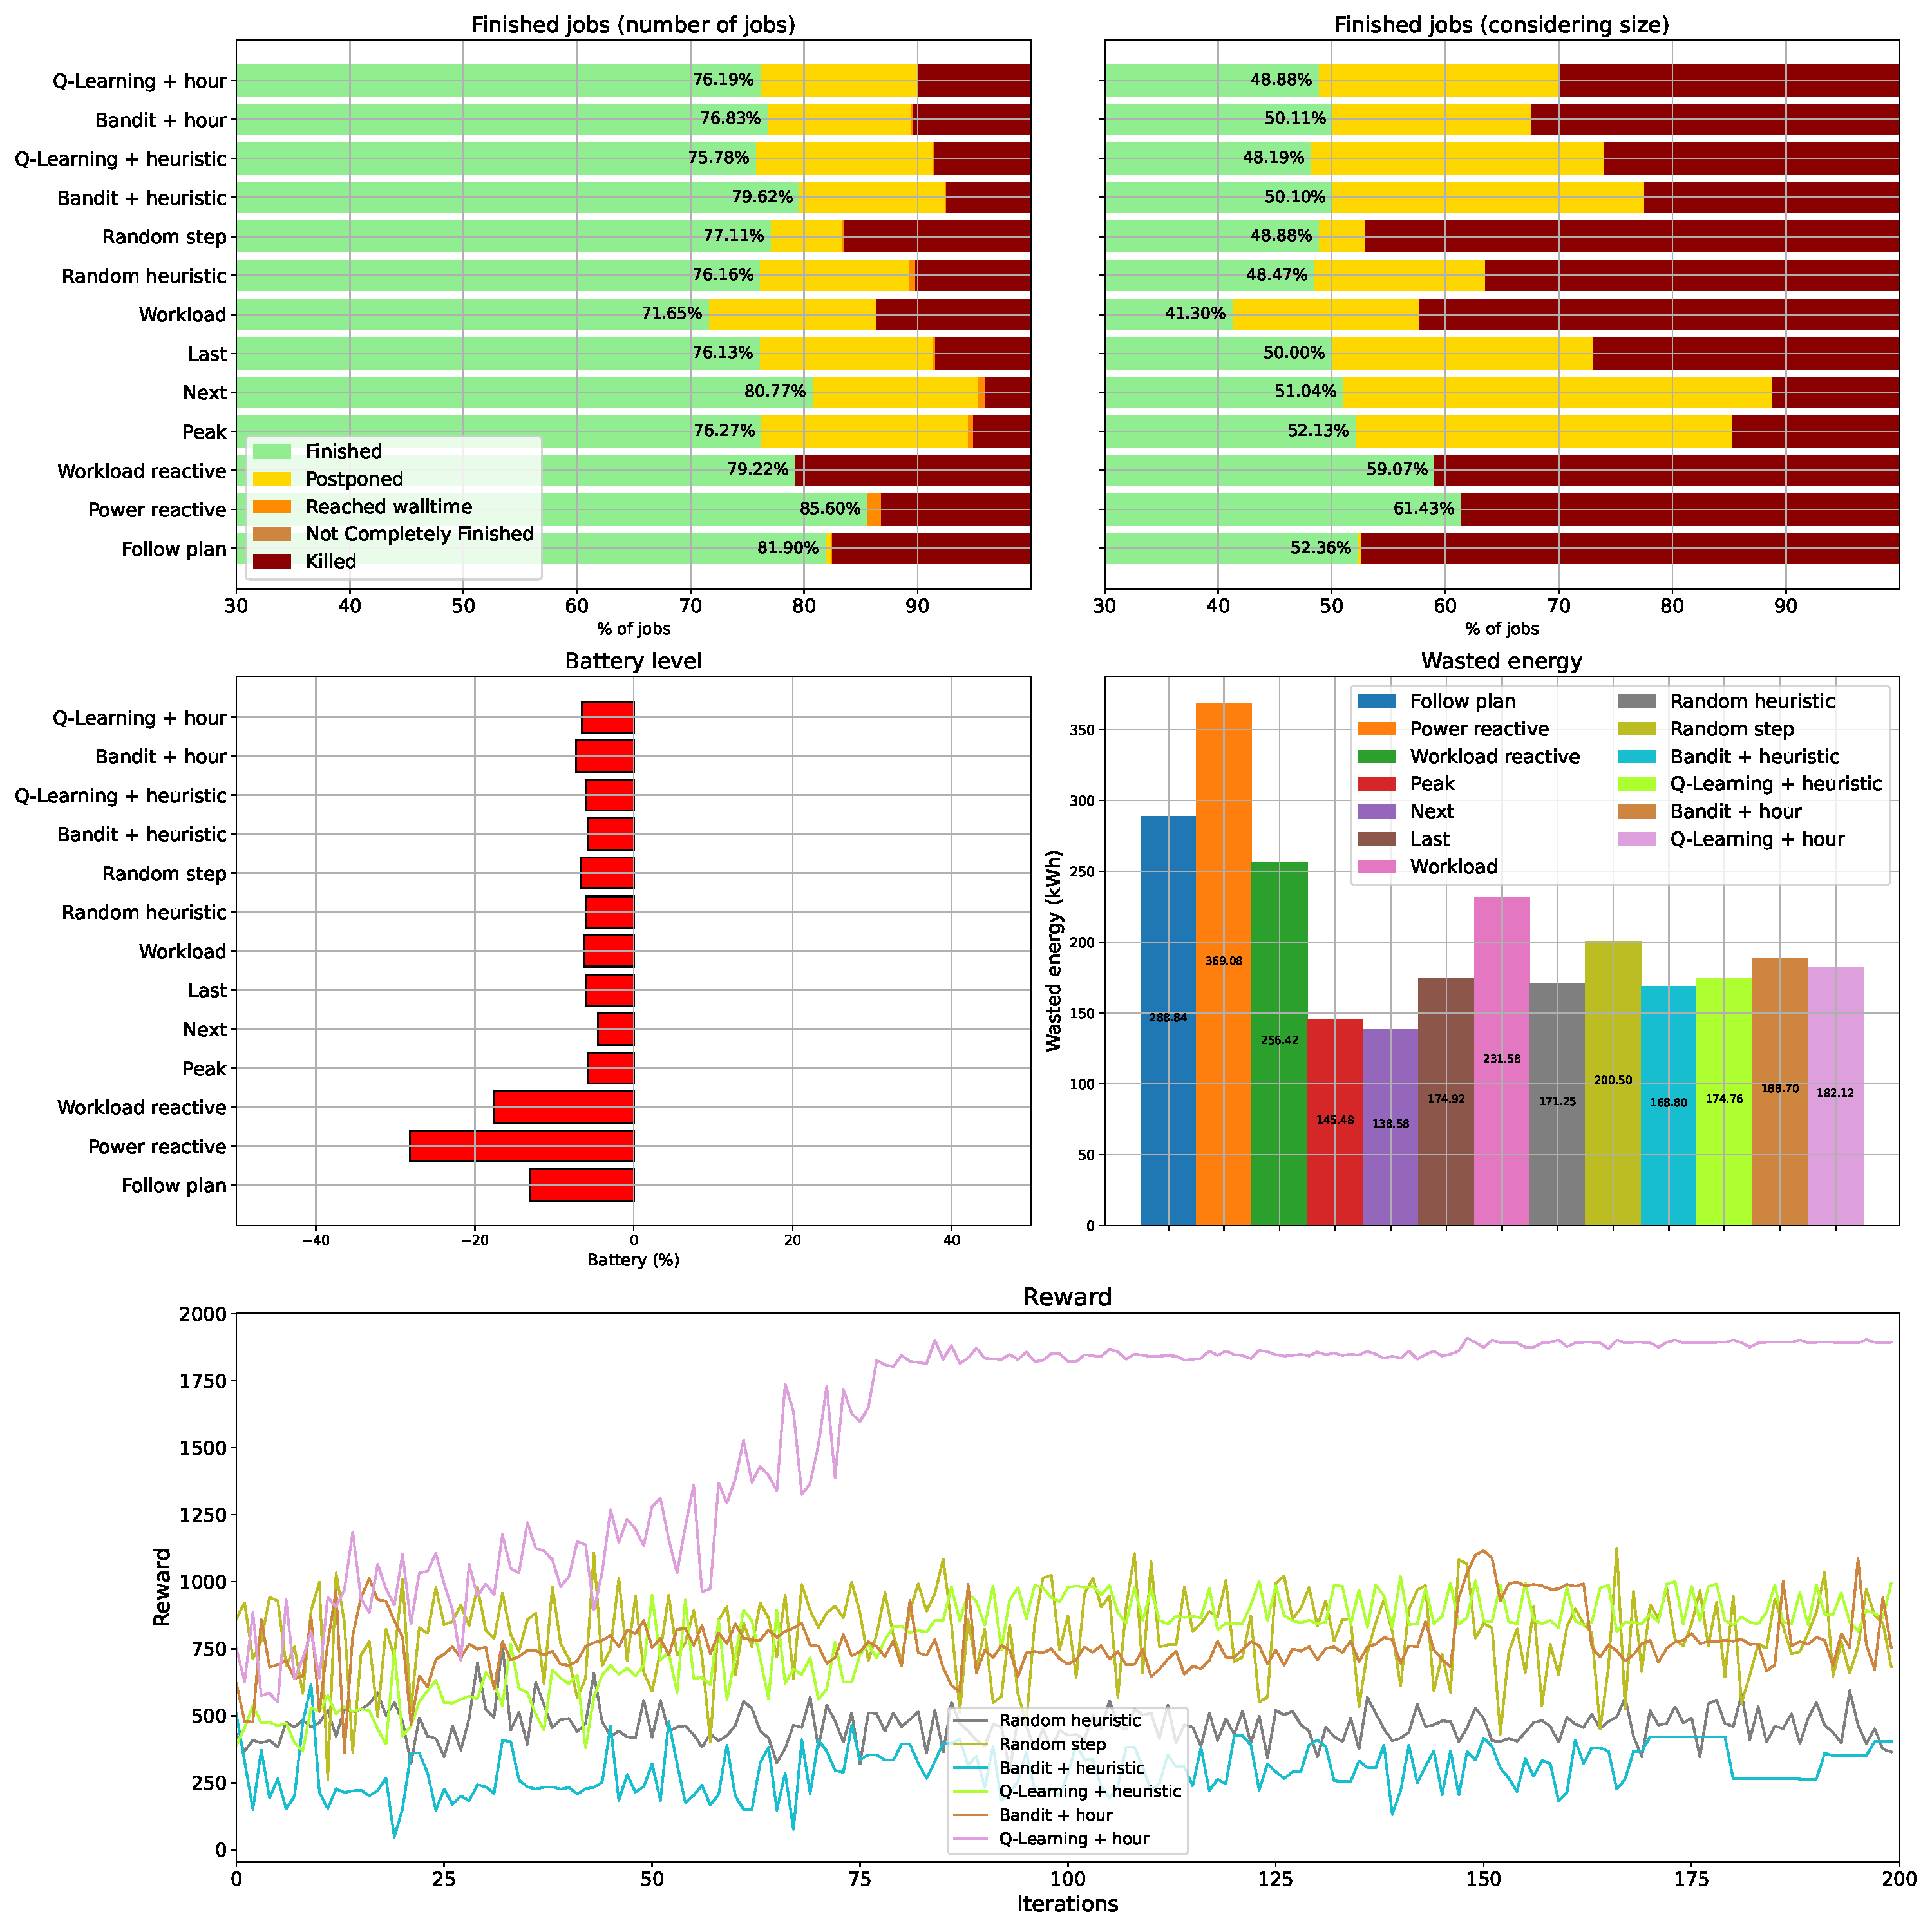
\includegraphics[scale=0.29]{Images/Learning_compensations/reward_finished_touched_profile_worst_workload_1_with_noise_state_delta.pdf}
    \caption{Results of finished jobs reward in critical case 3.}
    \label{fig:touched_reward_results_critical_3}
\end{figure}

\begin{figure}[!htb]
    \centering
    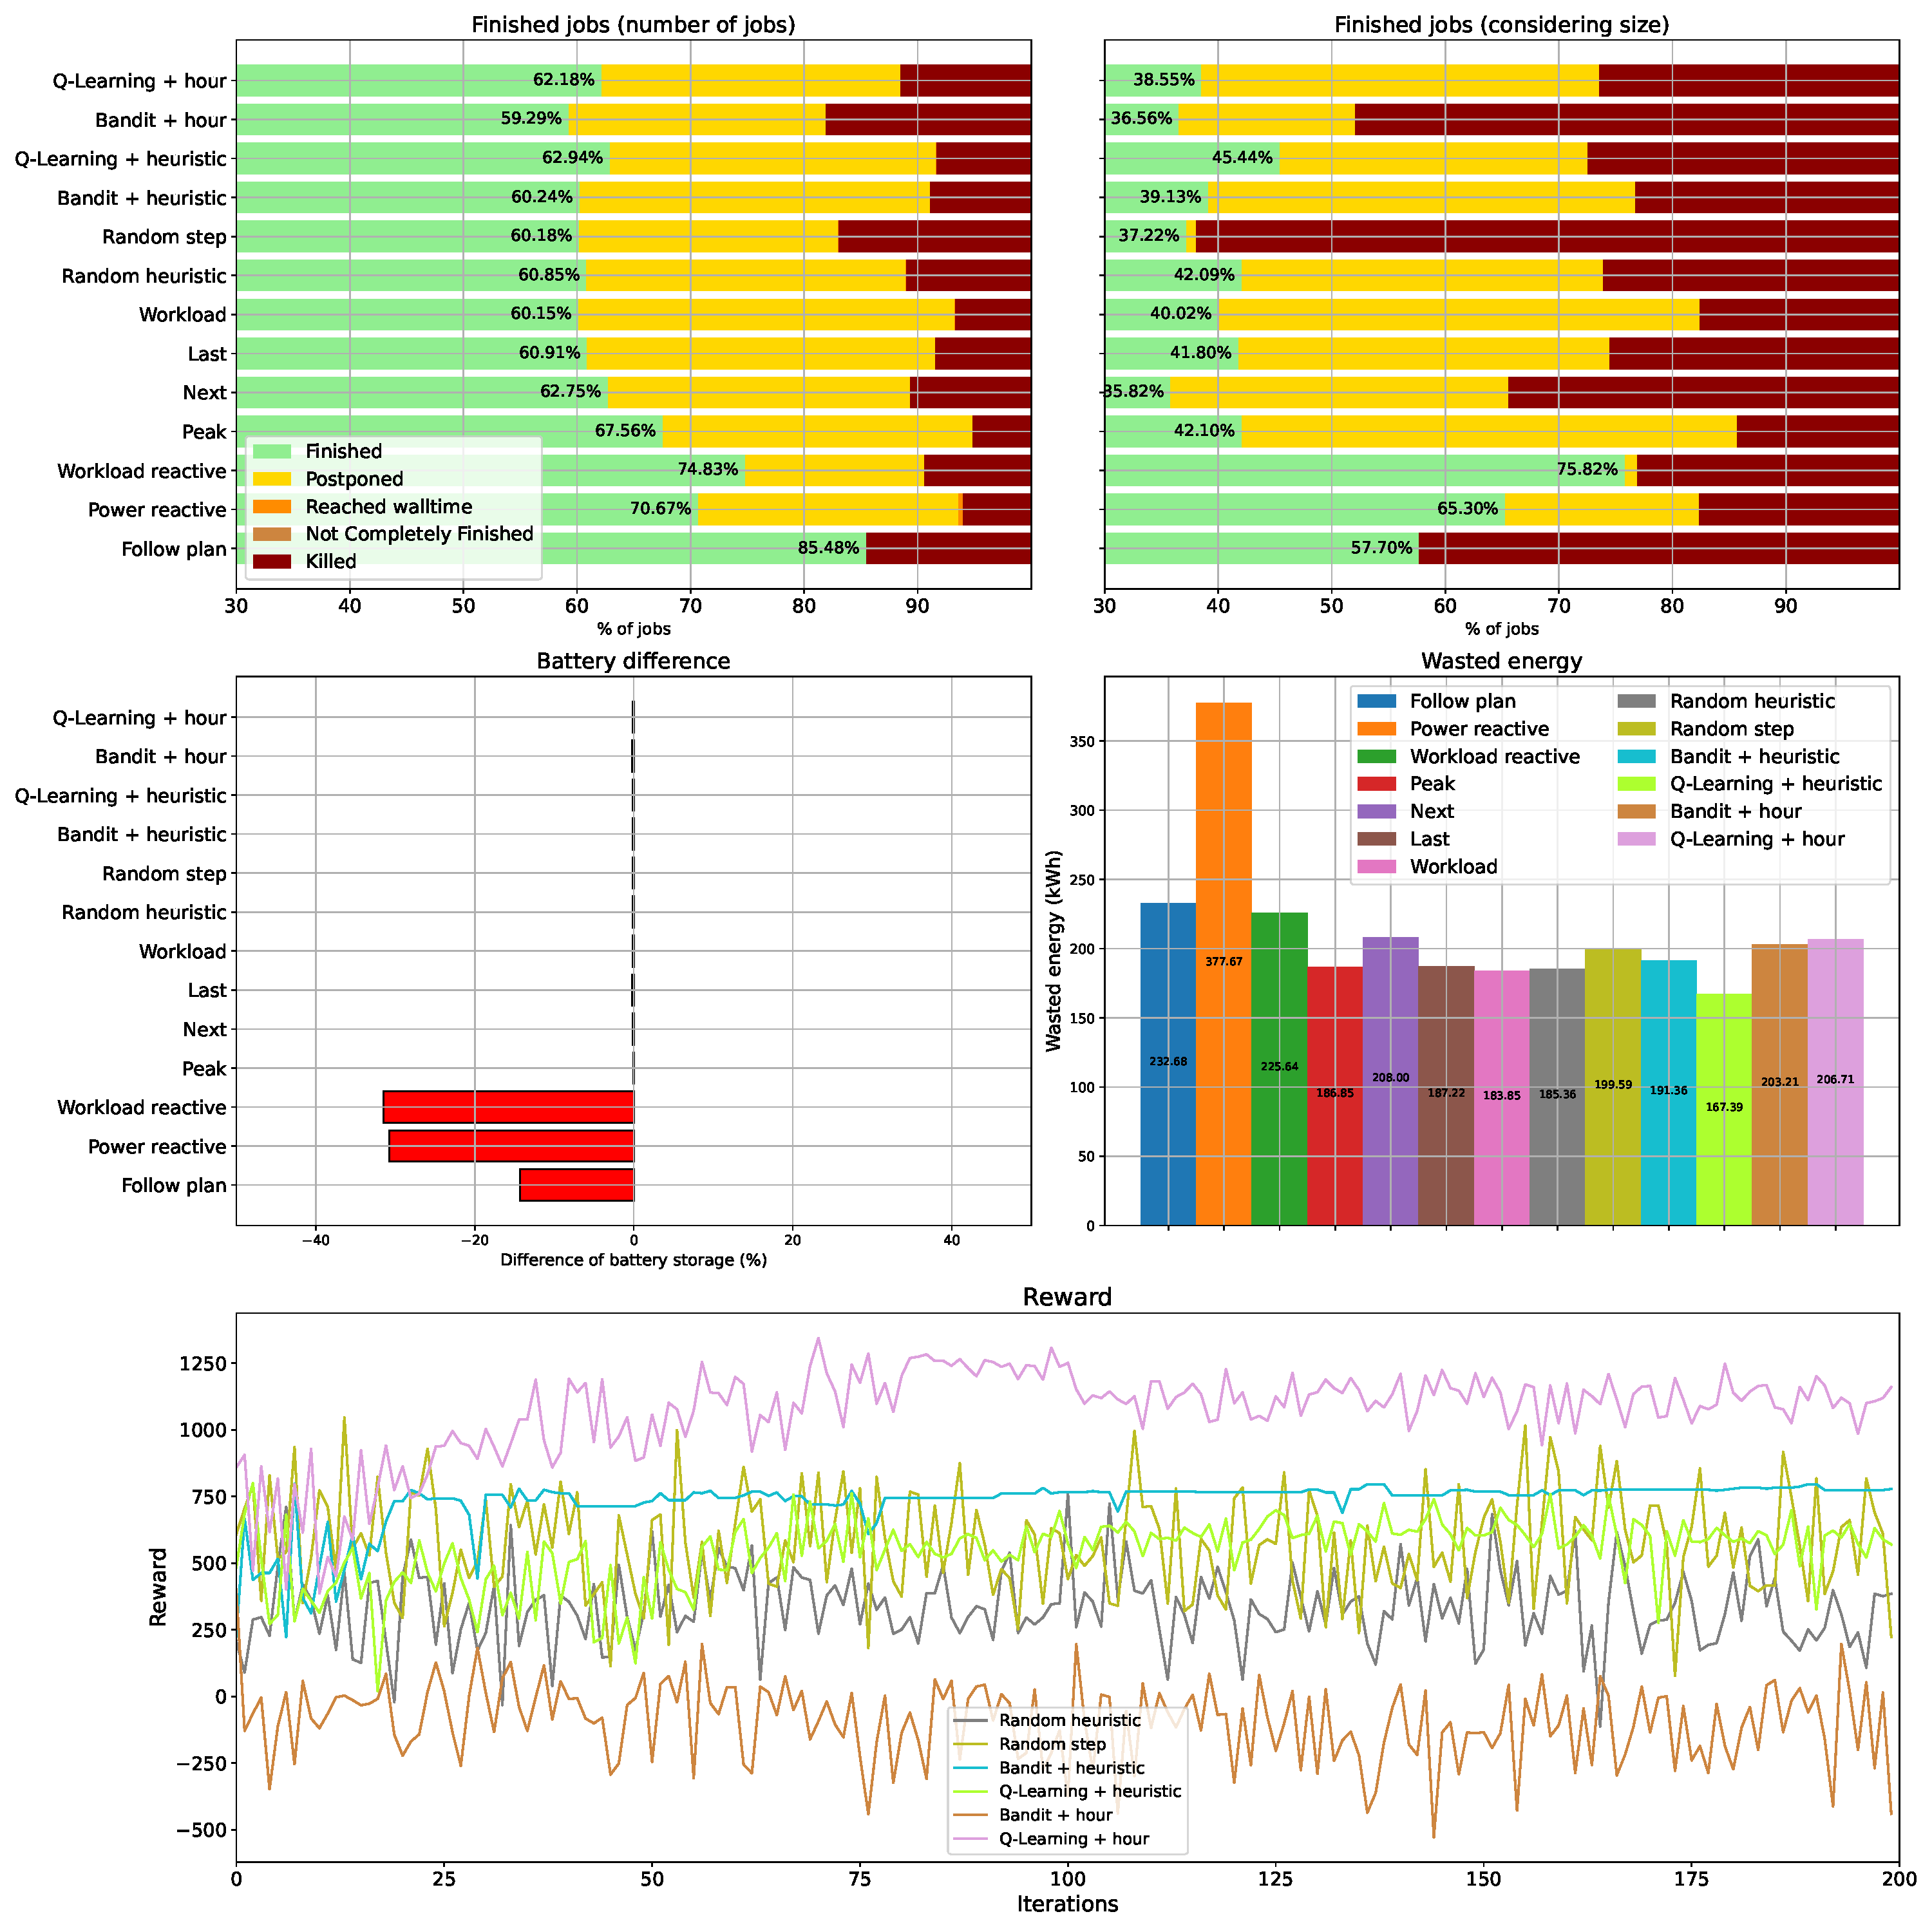
\includegraphics[scale=0.29]{Images/Learning_compensations/reward_finished_touched_profile_worst_workload_2_with_noise_state_delta.pdf}
    \caption{Results of finished jobs reward in critical case 4.}
    \label{fig:touched_reward_results_critical_4}
\end{figure}



% \clearpage

% \subsection{Finished Jobs Spread Reward}

% \begin{figure}[!htb]
%     \centering
%     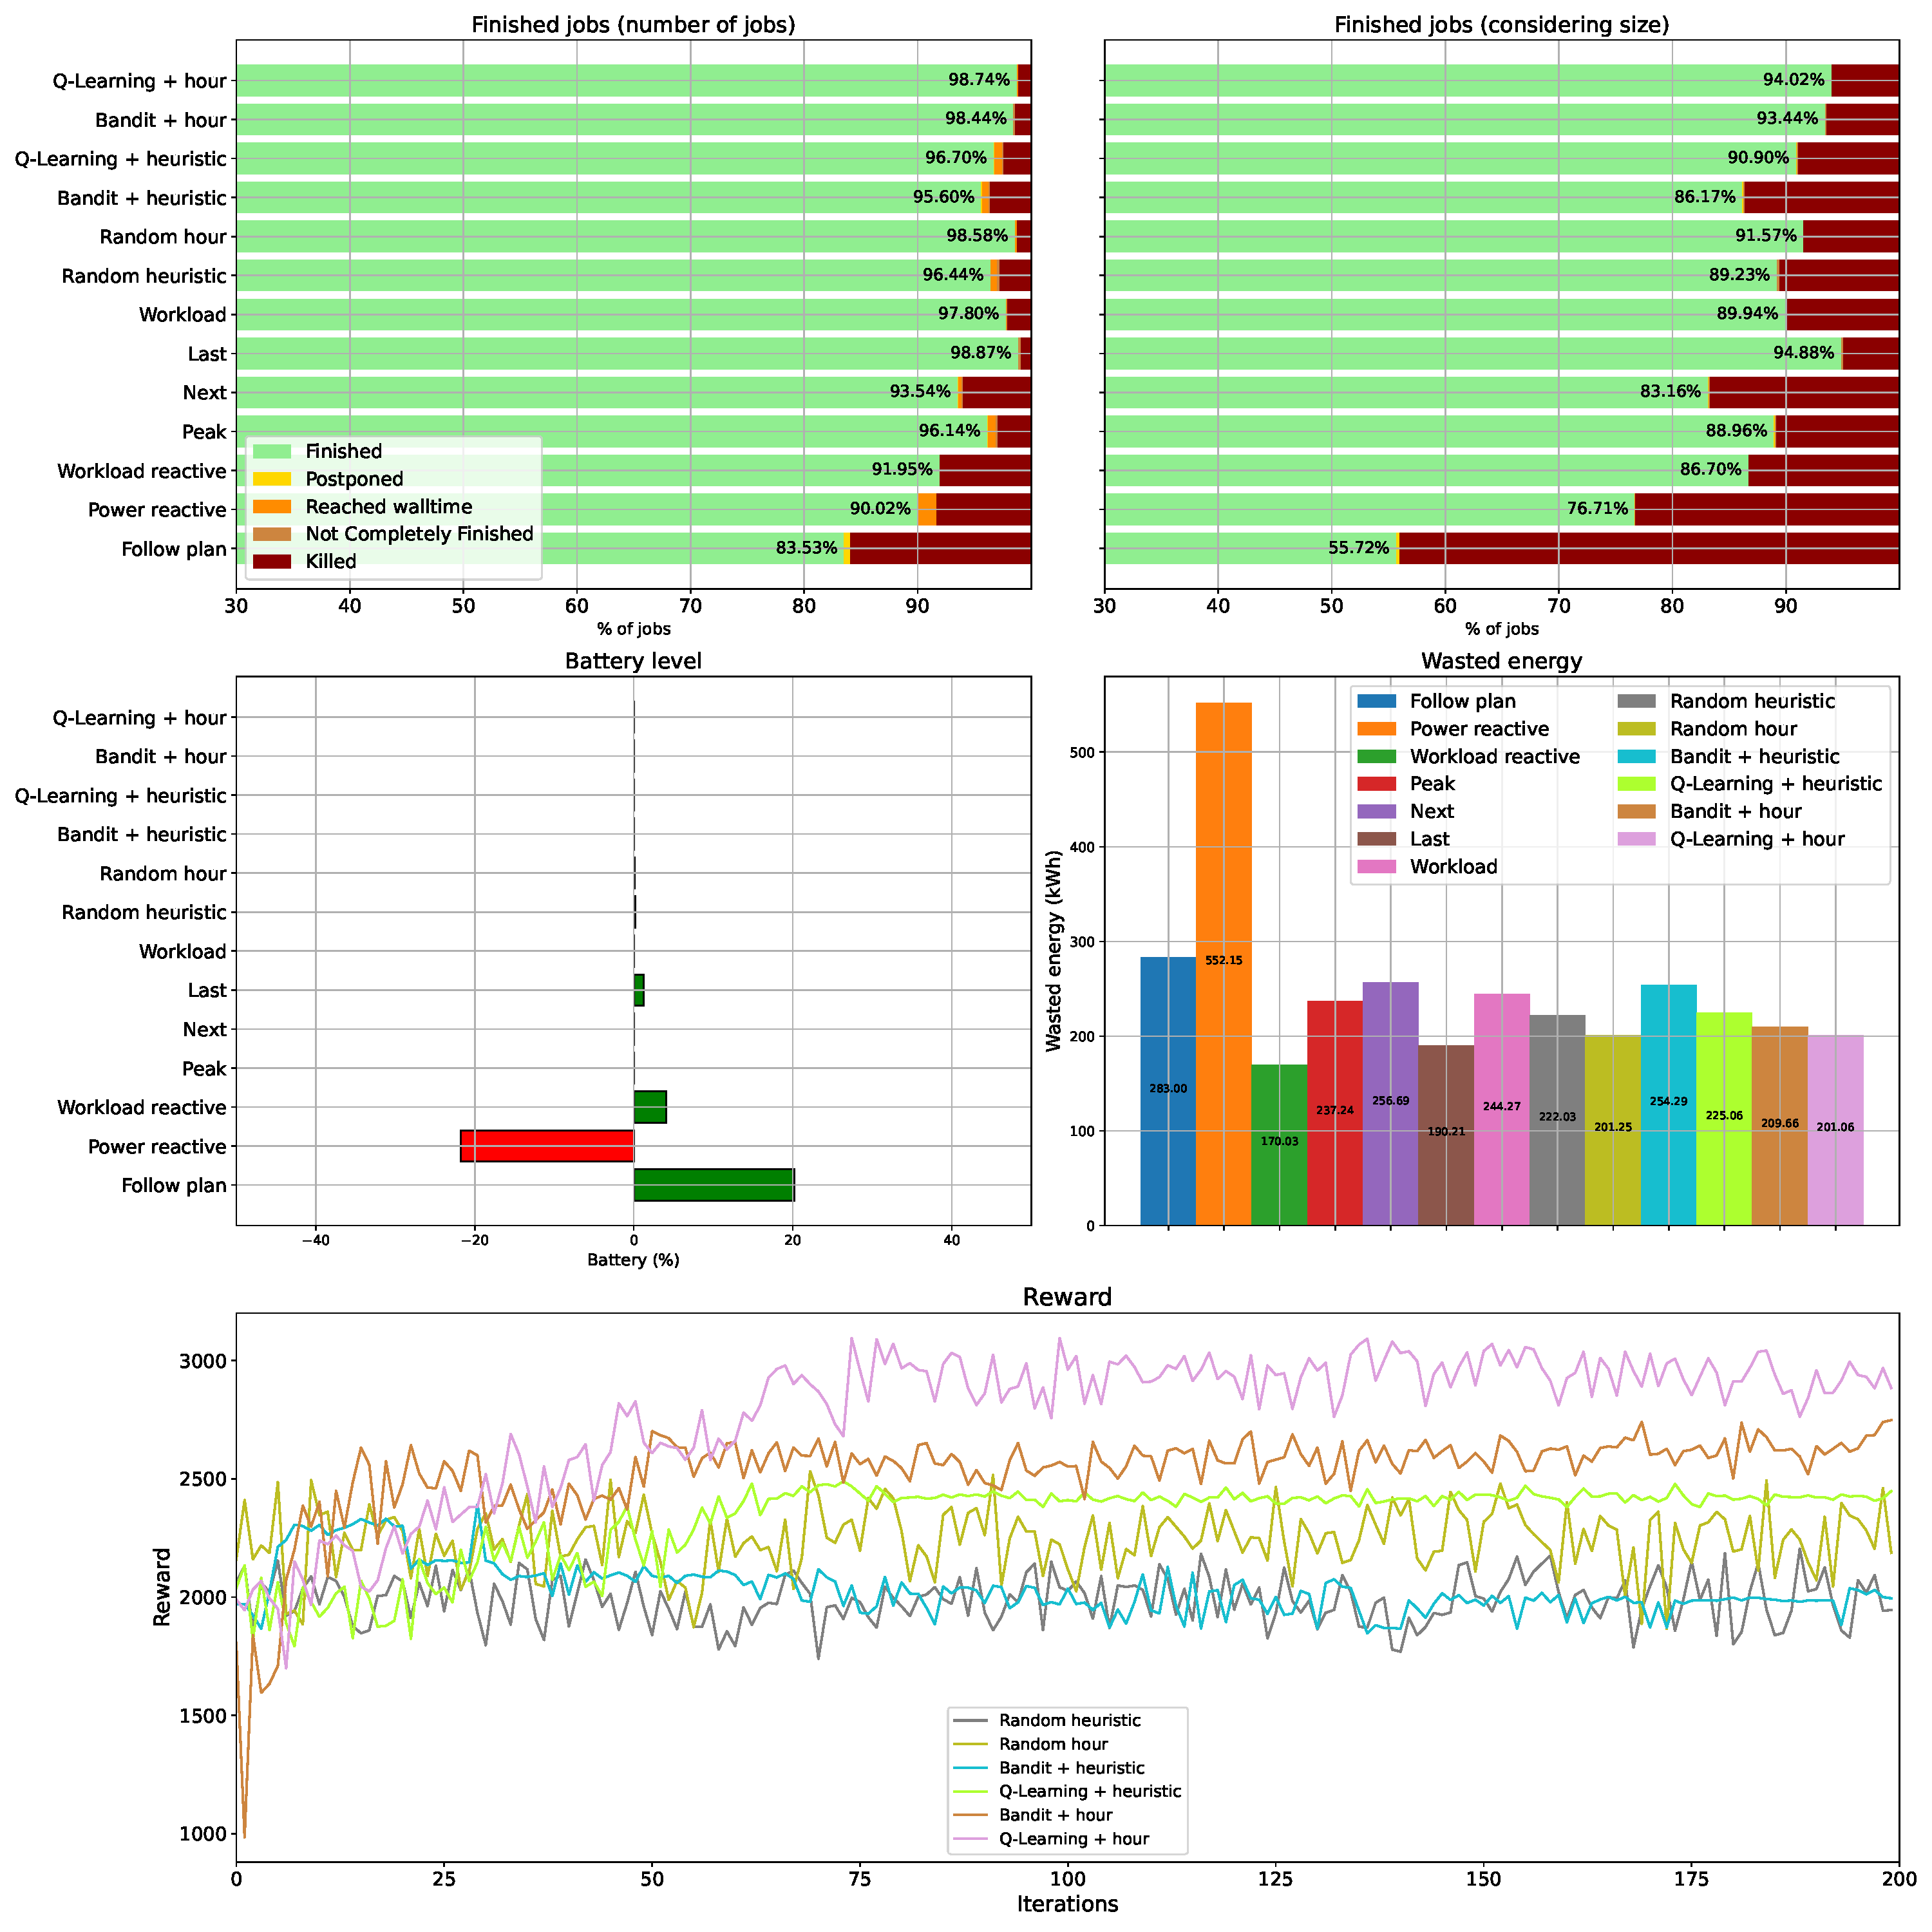
\includegraphics[scale=0.29]{Images/Learning_compensations/reward_finished_spread_profile_best_workload_1_with_noise_state_delta.pdf}
%     \caption{Results of reward finished jobs spread reward in critical case 1.}
%     \label{fig:spread_reward_results_critical_1}
% \end{figure}

% \begin{figure}[!htb]
%     \centering
%     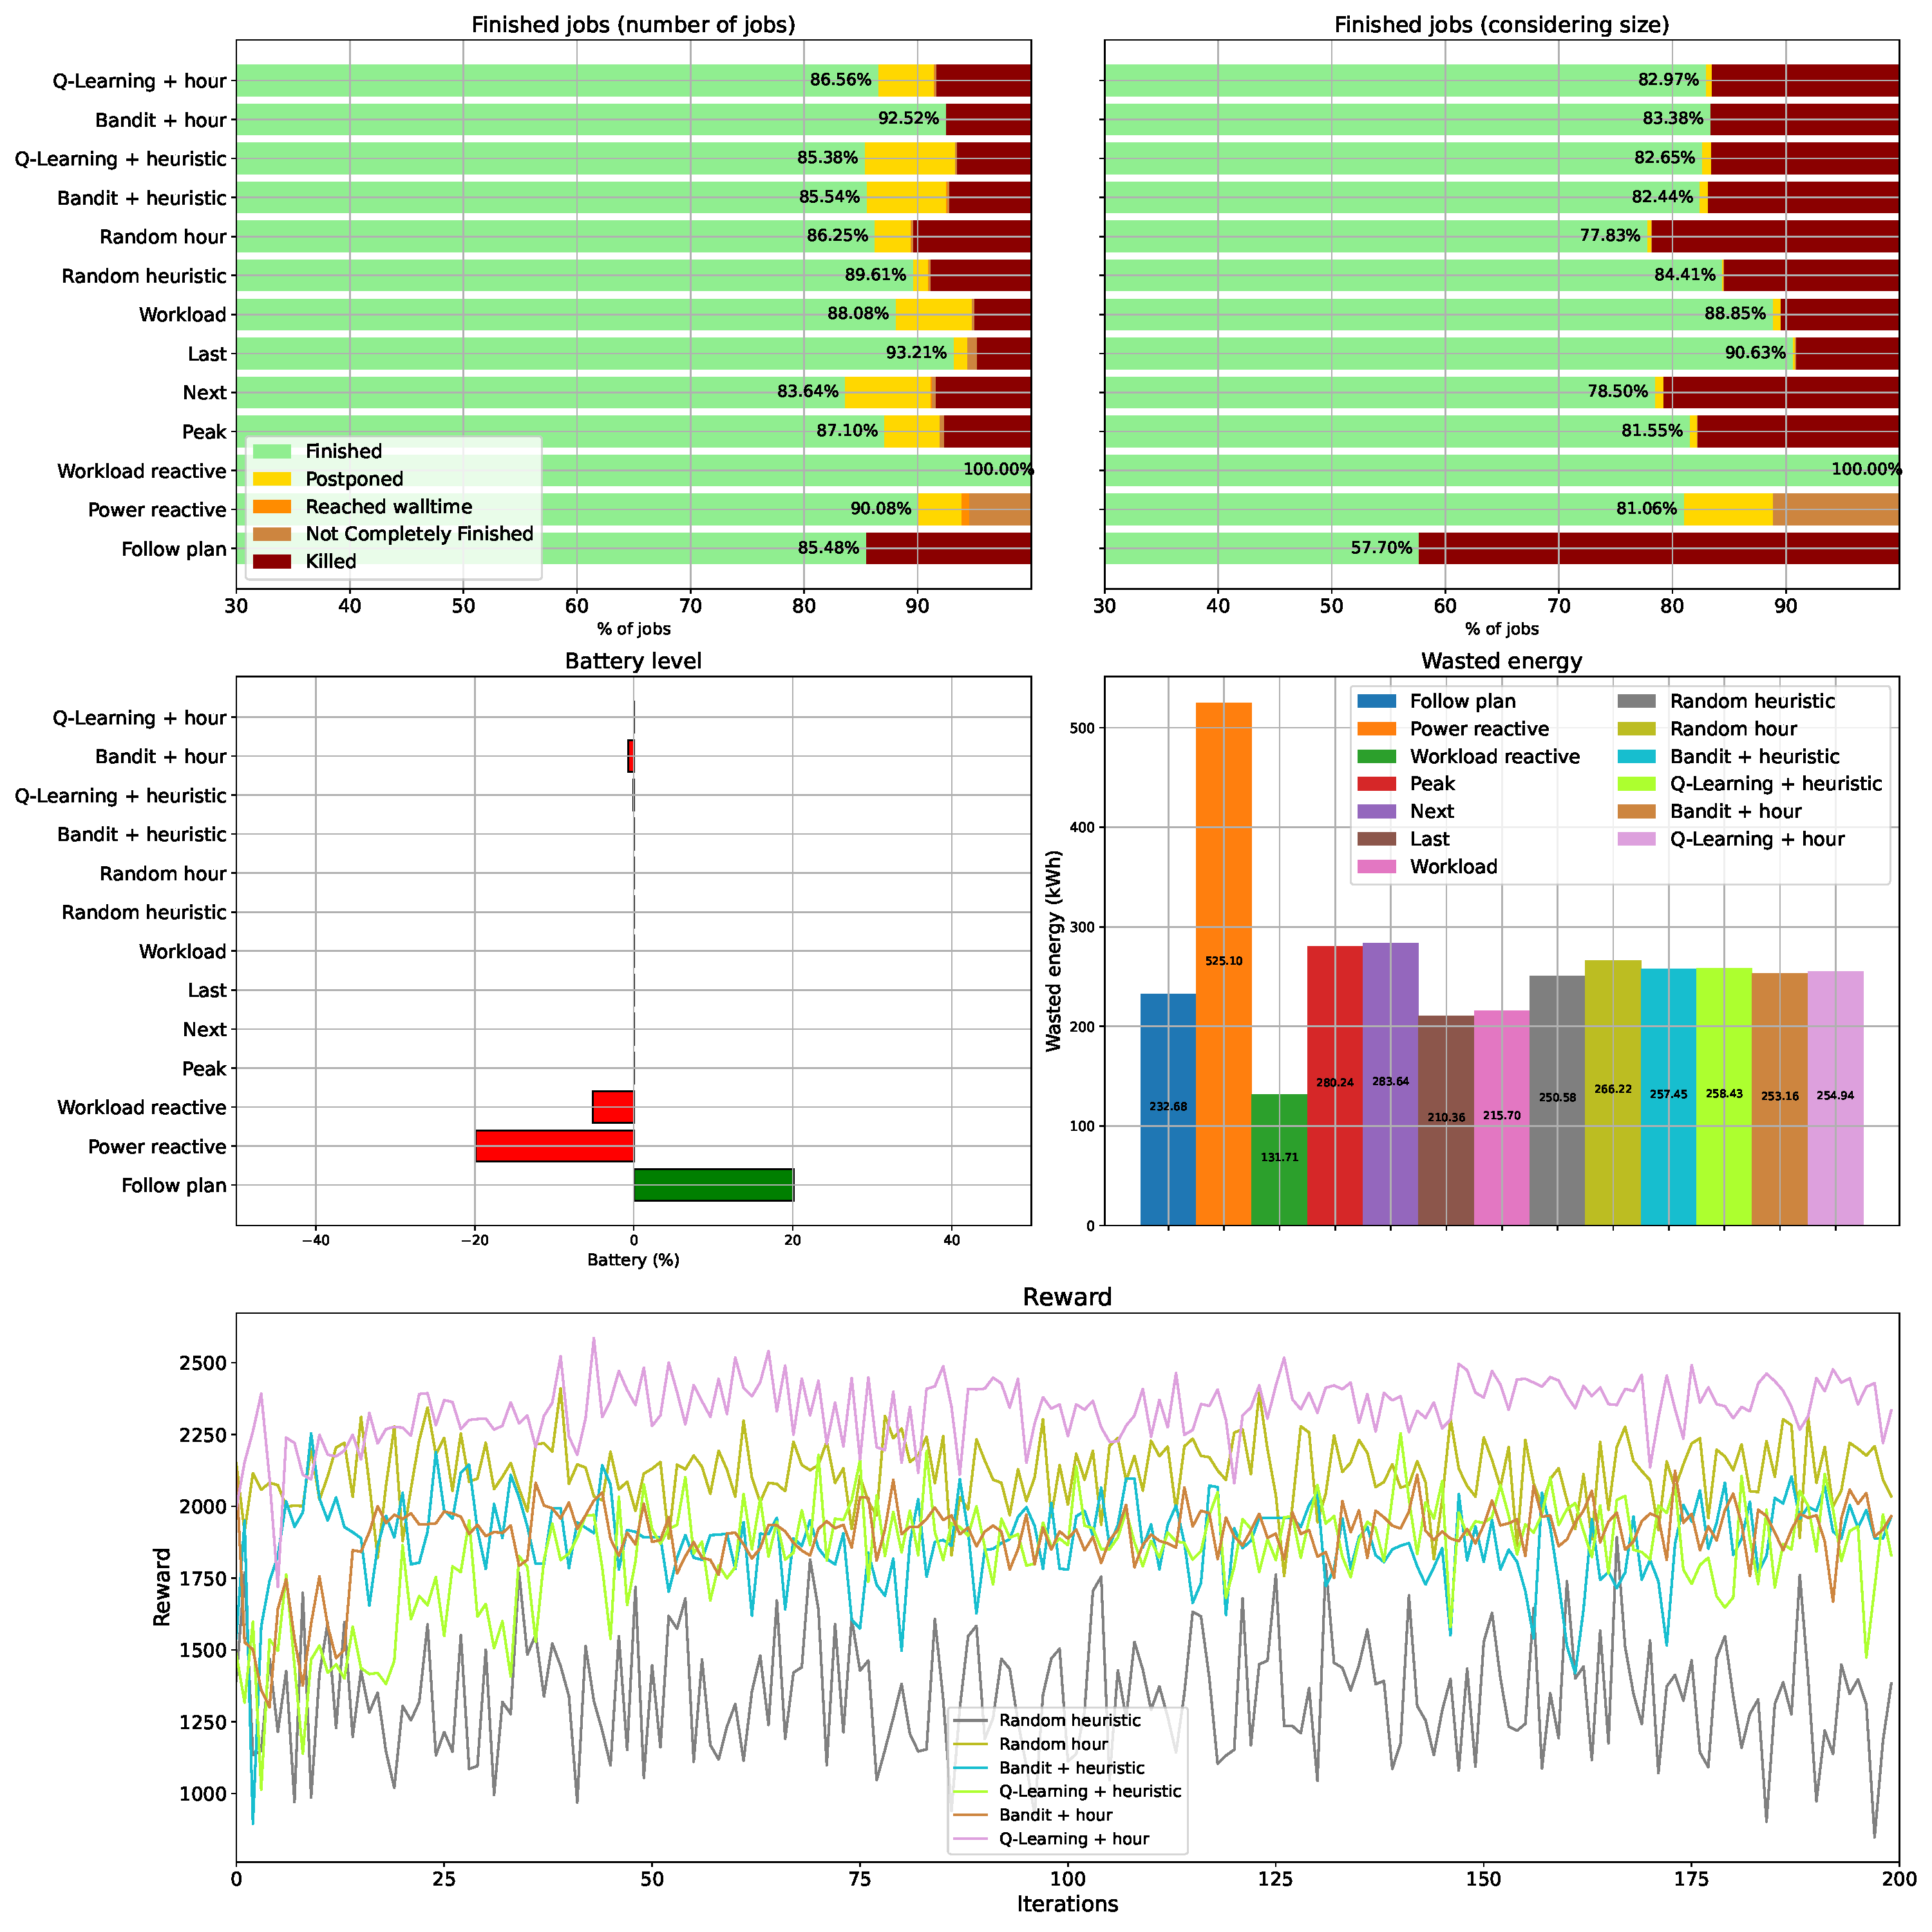
\includegraphics[scale=0.29]{Images/Learning_compensations/reward_finished_spread_profile_best_workload_2_with_noise_state_delta.pdf}
%     \caption{Results of reward finished jobs spread reward in critical case 2.}
%     \label{fig:spread_reward_results_critical_2}
% \end{figure}

% \begin{figure}[!htb]
%     \centering
%     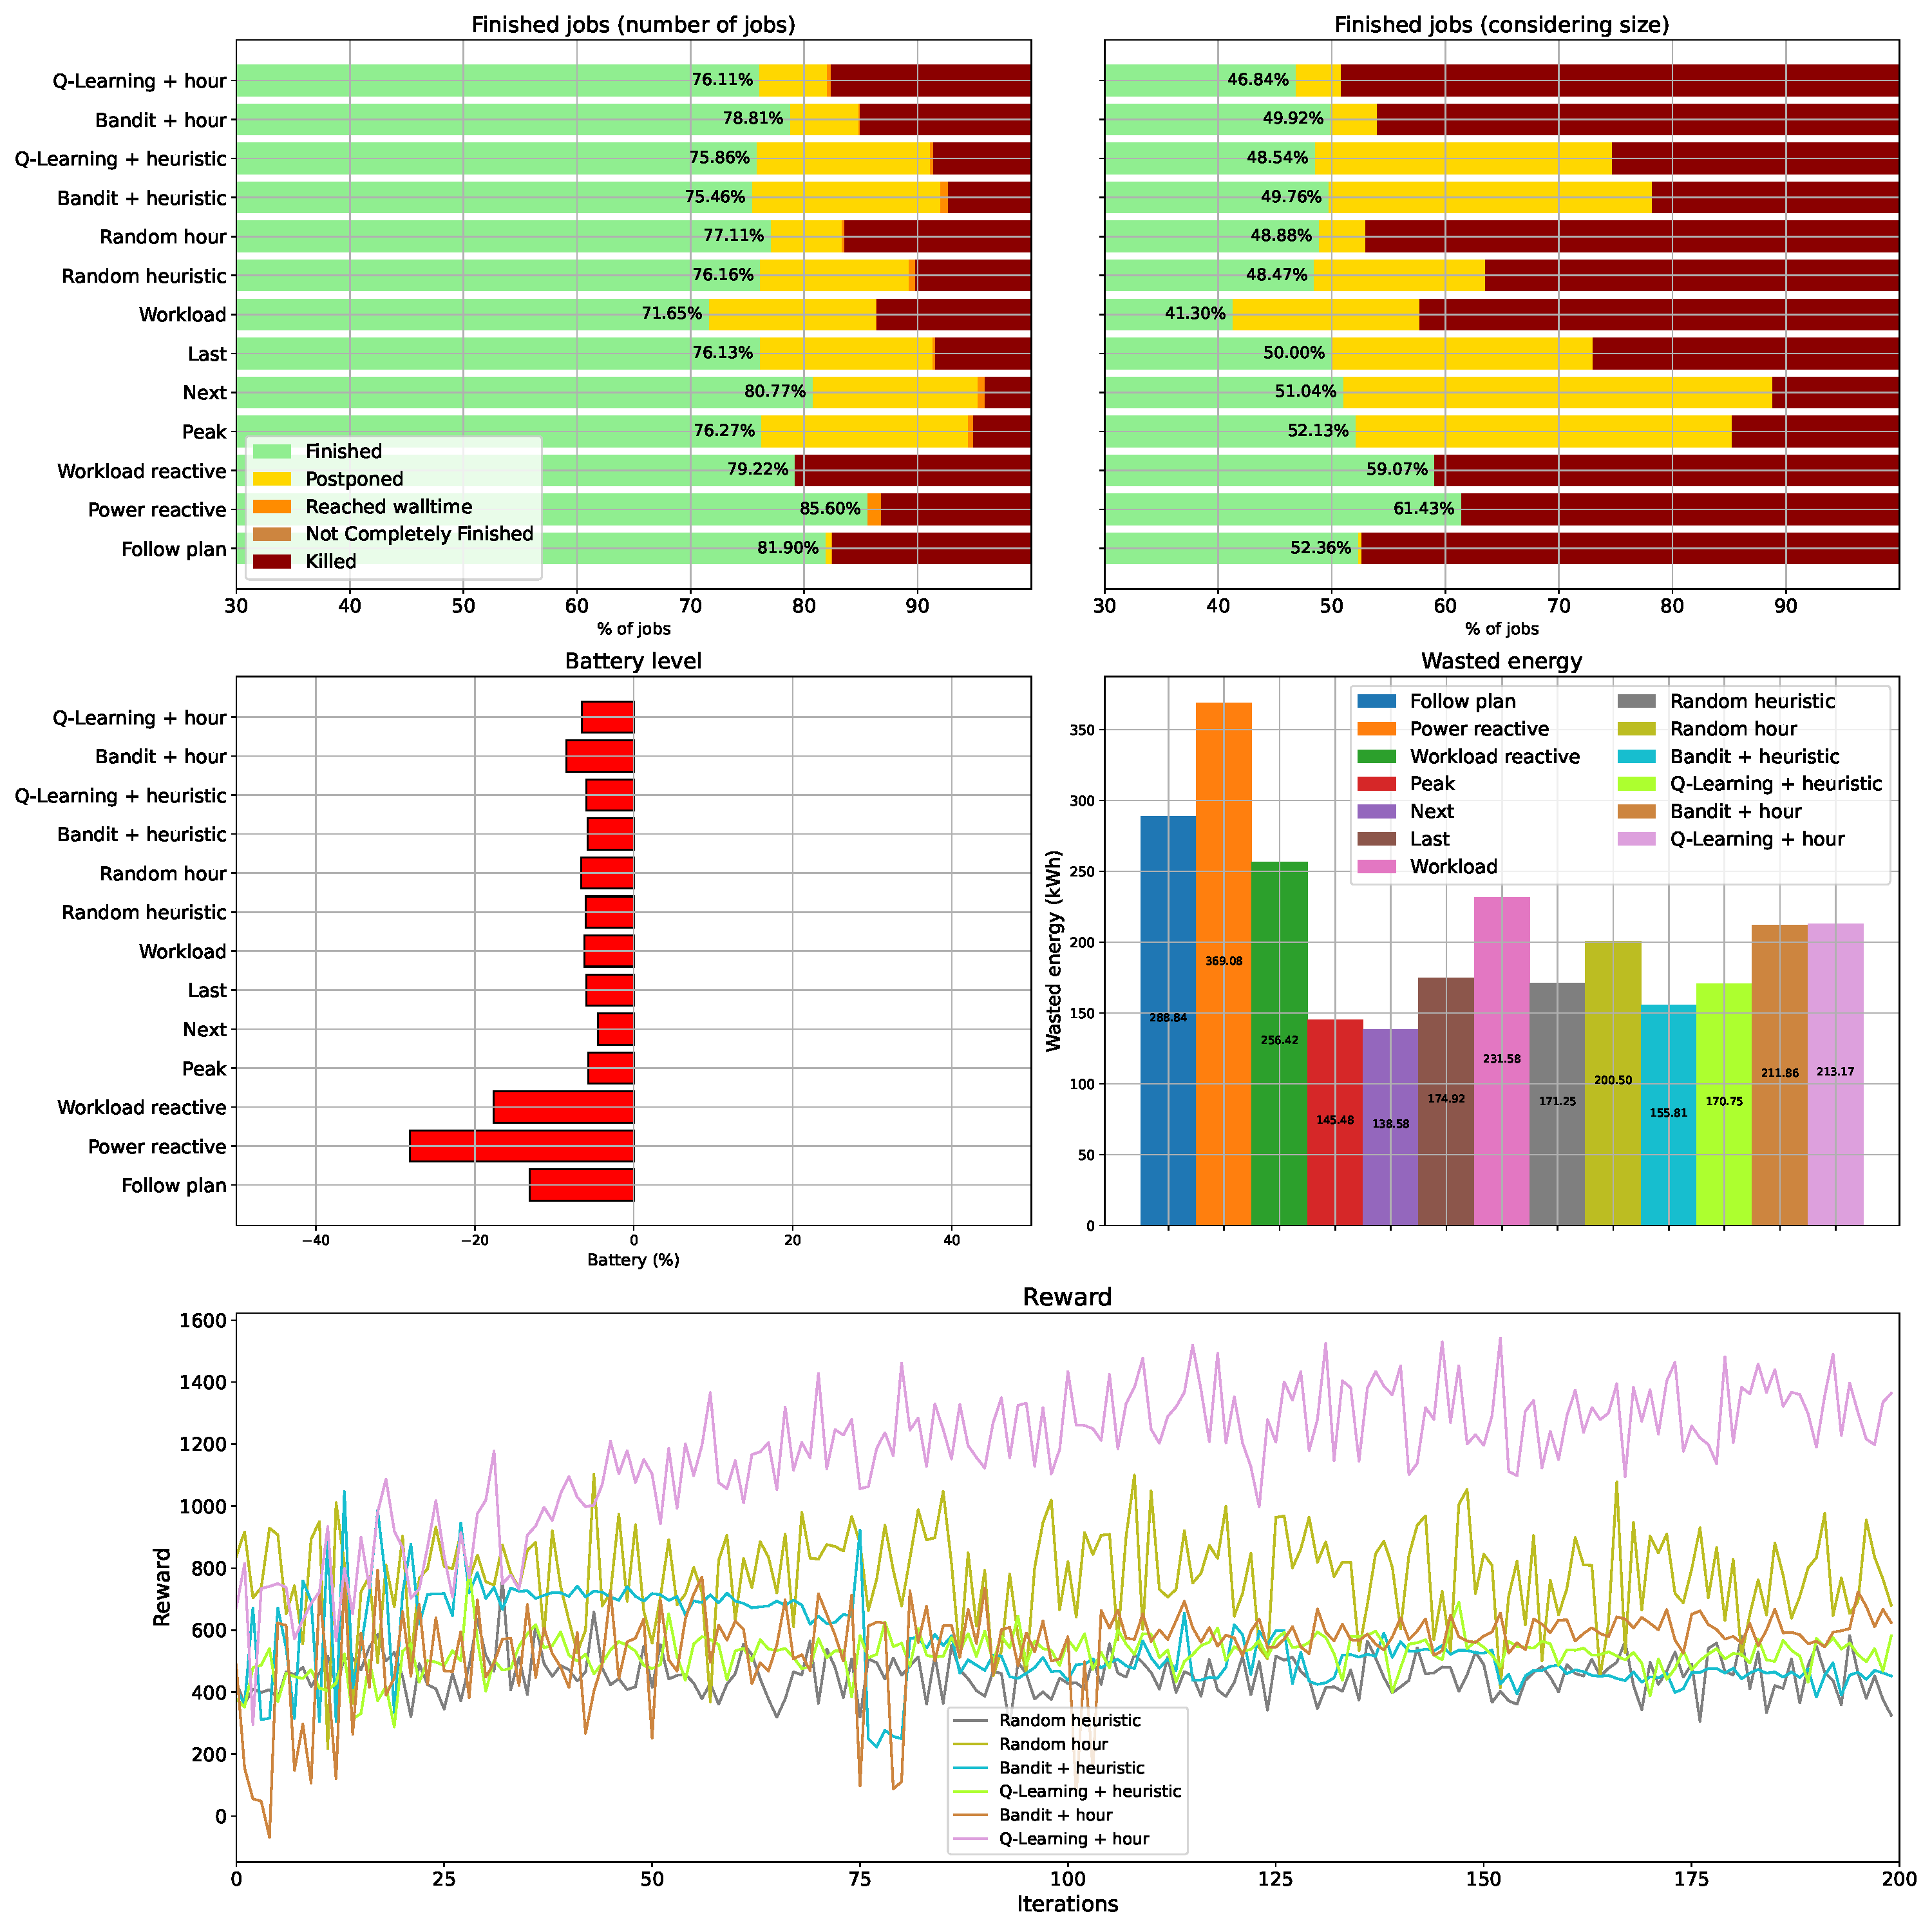
\includegraphics[scale=0.29]{Images/Learning_compensations/reward_finished_spread_profile_worst_workload_1_with_noise_state_delta.pdf}
%     \caption{Results of reward finished jobs spread reward in critical case 3.}
%     \label{fig:spread_reward_results_critical_3}
% \end{figure}

% \begin{figure}[!htb]
%     \centering
%     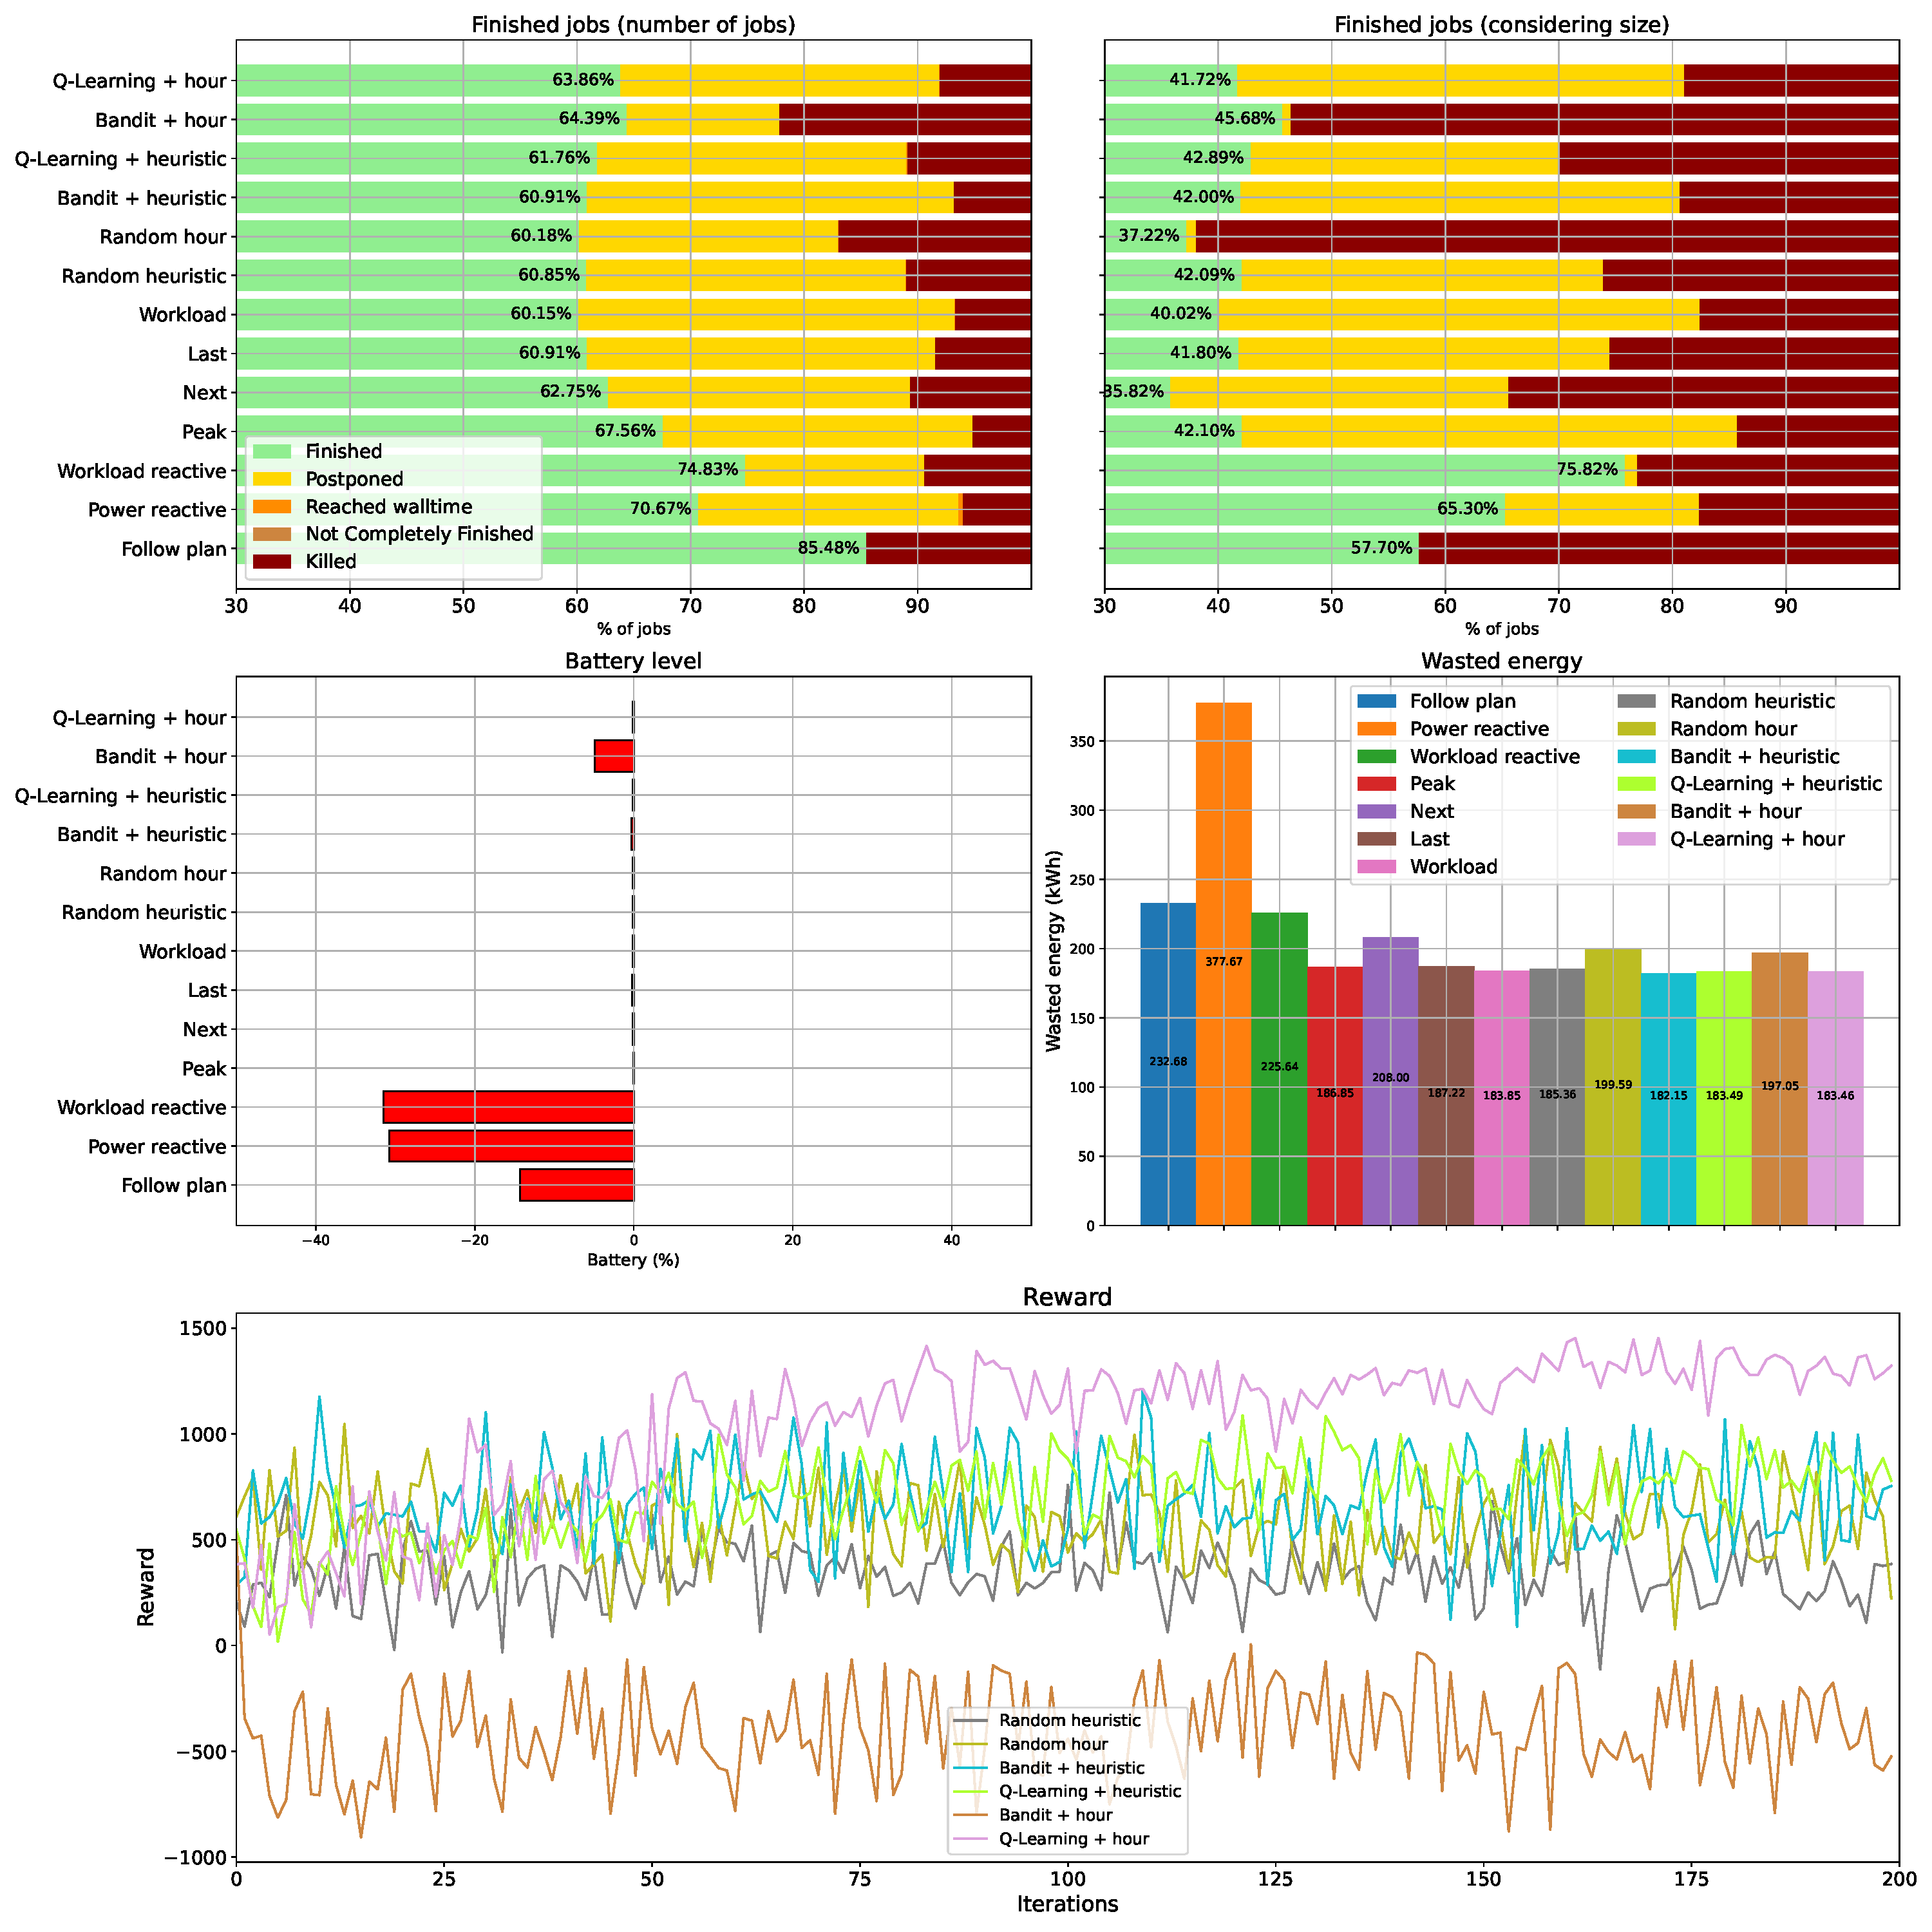
\includegraphics[scale=0.29]{Images/Learning_compensations/reward_finished_spread_profile_worst_workload_2_with_noise_state_delta.pdf}
%     \caption{Results of reward finished jobs spread reward in critical case 4.}
%     \label{fig:spread_reward_results_critical_4}
% \end{figure}

\clearpage

\subsection{Discussion}

\section{Conclusion}